\documentclass[landscape]{uedslides2C}
\usepackage{url}
\usepackage{amsmath}
\usepackage{graphicx}
\usepackage{color}
\usepackage{colortbl}
\usepackage{epic,ecltree}
%\usepackage{bar}
\usepackage{eclbip}
\usepackage{fancybox}
%\usepackage{pause} % java -jar ~/Code/statmt/bin/pp4p.jar mtsummit09-talk.pdf mtsummit09-talk.view.pdf
\usepackage{pdfpages}
\usepackage{fancyvrb}
\usepackage[absolute]{textpos}
\renewcommand*\ttdefault{txtt} % 20% tighter than courier
\usepackage{tikz}
%\usepackage{tikz-qtree}
\usepackage{natbib}
\usetikzlibrary{arrows,shapes}
%\usepackage[english,vietnam]{babel}
%\usepackage[utf8]{inputenc}
\usepackage{multicol}
\usepackage{tikz}
\usepackage{tikz-qtree}
\usepackage{multirow}
\usepackage{rotating}
\usepackage[absolute]{textpos}

\definecolor{lightblue}{rgb}{.8,.8,1}
\definecolor{mediumlightblue}{rgb}{.5,.5,1}
\definecolor{lightyellow}{rgb}{1,1,.5}
\definecolor{lightorange}{rgb}{1,.9,.7}
\definecolor{darkorange}{rgb}{1,.75,.2}
\definecolor{verydarkorange}{rgb}{.5,.3,0}
\definecolor{darkblue}{rgb}{0,0,0.8}
\definecolor{verydarkgreen}{rgb}{0,0.4,0}
\definecolor{darkgreen}{rgb}{0,0.8,0}
\definecolor{lightgreen}{rgb}{.8,1,.8}
\definecolor{lightred}{rgb}{1,.8,.8}
\definecolor{gray}{rgb}{0.9,0.9,0.9}
\definecolor{darkgrey}{rgb}{0.5,0.5,0.5}
\definecolor{verydarkgrey}{rgb}{0.3,0.3,0.3}
\definecolor{purple}{rgb}{0.6,0,0.6}
\definecolor{red}{rgb}{1,0,0}
\definecolor{orange}{rgb}{.8,.6,0}
\definecolor{cyan}{rgb}{0,.6,.6}

\newcommand{\newconcept}[1]{\textcolor{blue}{\bf #1}}
\newcommand{\example}[1]{\textcolor{darkblue}{\rm #1}}
\newcommand{\important}[1]{\textcolor{darkblue}{\em #1}}
\newcommand{\concept}[1]{\textcolor{darkblue}{\em #1}}
\newcommand{\maths}[1]{\textcolor{purple}{#1}}
\newcommand{\reference}[1]{\vspace{-2mm}\begin{flushright}\textcolor{purple}{\tiny [from #1]}\end{flushright}\vspace{-7mm}}

\newcommand{\highlightbox}[6]{\begin{textblock}{#3}(#1,#2) \colorbox{#4}{\textcolor{#5}{\begin{minipage}{#3in} #6 \end{minipage} }} \end{textblock}}
\newcommand{\backgroundbox}[5]{\highlightbox{#1}{#2}{#3}{#5}{black}{\vspace{#4in}\hspace{#3in}}}
\newcommand{\currenttopic}[1]{\colorbox{lightyellow}{\textcolor{black}{\bf #1}}}
\newcommand{\littlecode}[1]{\colorbox{gray}{\textcolor{black}{\small \tt #1}}}

\newcommand{\highlight}[1]{\colorbox{lightyellow}{#1}}
\newcommand{\highlightOrange}[1]{\colorbox{lightorange}{#1}}
\newcommand{\highlightGreen}[1]{\colorbox{lightgreen}{#1}}
\newcommand{\highlightBlue}[1]{\colorbox{lightblue}{#1}}

\bibliography{mt,more}

\begin{document}
\title[Machine Translation with Open Source Software]{{\sc \huge Moses}\\[3mm] Machine Translation with Open Source Software}
\author[Junczys-Dowmunt and Hoang]{Marcin Junczys-Dowmunt and Hieu Hoang}
\date{\vspace{-5mm}2 July 2014}
\maketitle

%%%%%%%%%%%%%%%%%%%%%%%%%%%%%%%%%%%%%%%%%%%%%%%%%%%%%%%%%%%%%%%%%%%%%%%%%%%%
% Introduction

\slide{Outline}
\vspace{20mm}

\begin{description}
\item[\small 09:30-10:00 $\;\;$] {\bf Introduction}
\item[\small 11:00-11:30 $\;\;$] Break
\item[\small 11:30-12:30 $\;\;$] {\bf Advanced Topics}
\end{description}

%%%%%%%%%%%%%%%%%%%%%%%%%%%%%%%%%%%%%%%%%%%%%%%%%%%%%%%%%%%%%%%%%%%%%%%%%%%%

\slide{Basic Idea}
\vspace{15mm}
\begin{center}
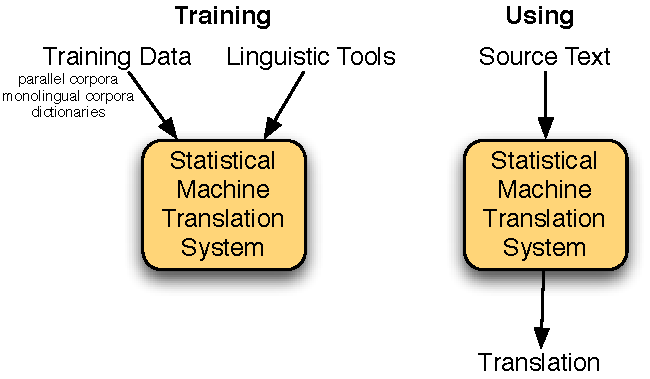
\includegraphics[scale=1.8]{basics.pdf}
\end{center}

%%%%%%%%%%%%%%%%%%%%%%%%%%%%%%%%%%%%%%%%%%%%%%%%%%%%%%%%%%%%%%%%%%%%%%%%%%%%

\slide{Statistical Machine Translation History}
\vspace{10mm}
\begin{description}
\item[around 1990] $\;$\\[2mm] Pioneering work at IBM, inspired by success in speech recognition
\item[1990s] $\;$\\[2mm] Dominance of IBM's word-based models, support technologies
\item[early 2000s] $\;$\\[2mm] Phrase-based models
\item[late 2000s] $\;$\\[2mm] Tree-based models
\end{description}

%%%%%%%%%%%%%%%%%%%%%%%%%%%%%%%%%%%%%%%%%%%%%%%%%%%%%%%%%%%%%%%%%%%%%%%%%%%%

\slide{Moses History}
\begin{description} \itemsep -0.2mm
\item[2002] $\;$ Pharaoh decoder, precursor to Moses (phrase-based models)
\item[2005] $\;$ Moses started by Hieu Hoang and Philipp Koehn (factored models)
\item[2006] $\;$ JHU workshop extends Moses significantly
\item[2006-2012] $\;$ Funding by EU projects EuroMatrix, EuroMatrixPlus
\item[2009] $\;$ Tree-based models implemented in Moses
\item[2012-2015] $\;$ MosesCore project. Full-time staff to maintain and enhance Moses
\end{description}

%%%%%%%%%%%%%%%%%%%%%%%%%%%%%%%%%%%%%%%%%%%%%%%%%%%%%%%%%%%%%%%%%%%%%%%%%%%%

\slide{Moses in Academia}
\vspace{10mm}
\begin{itemize}
\item Built by academics, for academics
\item Reference implementation of state of the art
\begin{itemize}
\item researchers develop new methods on top of Moses
\item developers re-implement published methods
\item used by other researchers as black box
\end{itemize}
\item Baseline to beat
\begin{itemize}
\item researchers compare their method against Moses
\end{itemize}
\end{itemize}

%%%%%%%%%%%%%%%%%%%%%%%%%%%%%%%%%%%%%%%%%%%%%%%%%%%%%%%%%%%%%%%%%%%%%%%%%%%%

\slide{Developer Community}
\begin{itemize} \itemsep -1mm
\item Main development at University of Edinburgh, but also: \vspace{-3mm}
\begin{itemize}
\item Fondazione Bruno Kessler (Italy)
\item Charles University (Czech Republic)
\item DFKI (Germany)
\item RWTH Aachen (Germany)
\item others...
\end{itemize}
\item Code shared on github.com
\item Main forum: support and developer mailing lists
\item Main event: Machine Translation Marathon (September in Trento, Italy)\vspace{-3mm}
\begin{itemize}
\item annual open source convention
\item presentation of new open source tools
\item hands-on work on new open source projects
\item summer school for statistical machine translation
\end{itemize}
\end{itemize}

%%%%%%%%%%%%%%%%%%%%%%%%%%%%%%%%%%%%%%%%%%%%%%%%%%%%%%%%%%%%%%%%%%%%%%%%%%%%

\slide{Open Source Components}
\vspace{10mm}
\begin{itemize}
\item Moses distribution uses external open source tools
\begin{itemize}
\item word alignment: {\sc giza++}, Berkeley aligner, FastAlign
\item language model: {\sc srilm}, {\sc irstlm}, {\sc randlm}, {\sc kenlm}
\item scoring: {\sc bleu}, {\sc ter}, {\sc meteor}
\end{itemize}
\item Other useful tools
\begin{itemize}
\item sentence aligner
\item syntactic parsers
\item part-of-speech taggers
\item morphological analyzers
\end{itemize}
\end{itemize}

%%%%%%%%%%%%%%%%%%%%%%%%%%%%%%%%%%%%%%%%%%%%%%%%%%%%%%%%%%%%%%%%%%%%%%%%%%%%

\slide{Other Open Source MT Systems}
\begin{itemize} \itemsep -3mm
\item {\bf Joshua} --- Johns Hopkins University\\
{\small \tt http://joshua.sourceforge.net/}
\item {\bf CDec} --- University of Maryland\\
{\small \tt http://cdec-decoder.org/}
\item {\bf Jane} --- RWTH Aachen\\
{\small \tt http://www-i6.informatik.rwth-aachen.de/jane/}
\item {\bf Phrasal} --- Stanford University\\
{\small \tt http://nlp.stanford.edu/phrasal/}
\item Very similar technology \vspace{-2mm}
\begin{itemize}
\item Joshua implemented in Java, others in C++
\item Joshua and Jane support only tree-based models
\item Phrasal supports only phrase-based models
\end{itemize}
\item Open sourcing tools increasing trend in NLP research
\end{itemize}

%%%%%%%%%%%%%%%%%%%%%%%%%%%%%%%%%%%%%%%%%%%%%%%%%%%%%%%%%%%%%%%%%%%%%%%%%%%%

\slide{Moses in Industry}
\vspace{20mm}
\begin{itemize}
\item Distributed with LGPL --- free to use
\item Competitive with commercial SMT solutions\\ (Language Weaver, Google, ...)
\item But:
\begin{itemize}
\item not easy to use
\item requires significant expertise for optimal performance
\item integration into existing workflow not straight-forward
\end{itemize}
\end{itemize}

%%%%%%%%%%%%%%%%%%%%%%%%%%%%%%%%%%%%%%%%%%%%%%%%%%%%%%%%%%%%%%%%%%%%%%%%%%%%

\slide{Case Studies}
\vspace{5mm}
\begin{description} \itemsep -1mm
\item[European Commission] ---\\  uses Moses in-house to aid human translators
\item[Autodesk] --- \\ showed productivity increases in translating manuals when post-editing output from a custom-build Moses system
\item[Systran] --- \\ developed statistical post-editing using Moses
\item[Asia Online] --- \\ offers translation technology and services based on Moses
\item[Many others] ... \\ World Trade Organisation, Adobe, Symantec, WIPO, Sybase, Safaba, Bloomberg, Pangeanic, KatanMT, Capita, ...

\end{description}


%%%%%%%%%%%%%%%%%%%%%%%%%%%%%%%%%%%%%%%%%%%%%%%%%%%%%%%%%%%%%%%%%%%%%%%%%%%%

\slide{Phrase-Based Model}
\begin{center} \vspace{15mm}
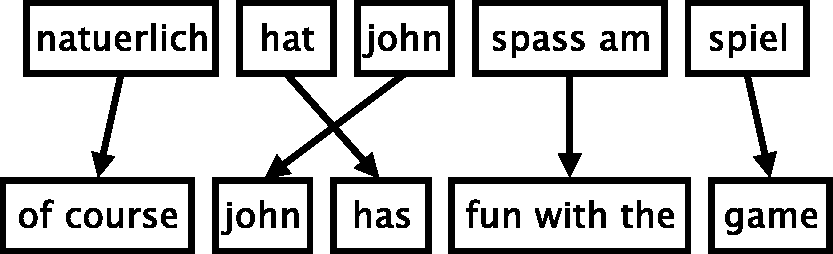
\includegraphics[scale=1.4]{phrase-model-alignment.pdf}
\end{center}\vspace{5mm}
\begin{itemize} \itemsep -1mm
\item Foreign input is segmented in phrases 
\item Each phrase is translated into English
\item Phrases are reordered
\end{itemize}

%%%%%%%%%%%%%%%%%%%%%%%%%%%%%%%%%%%%%%%%%%%%%%%%%%%%%%%%%%%%%%%%%%%%%%%%%%%%%

\slide{Phrase Translation Options}
\vspace{-5mm}
\begin{center} 
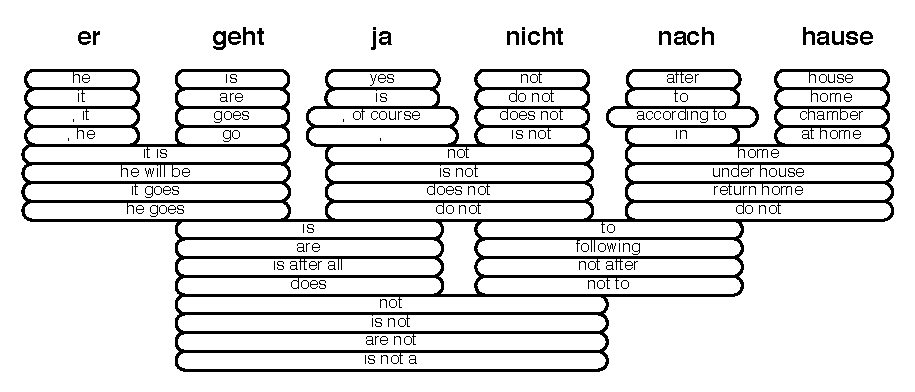
\includegraphics[scale=1.5]{translation-options.pdf}
\end{center}\vspace{-10mm}
\begin{itemize}
\item Many translation options to choose from
\end{itemize}

%%%%%%%%%%%%%%%%%%%%%%%%%%%%%%%%%%%%%%%%%%%%%%%%%%%%%%%%%%%%%%%%%%%%%%%%%%%%%

\slide{Phrase Translation Options}
\vspace{-5mm}
\begin{center} 
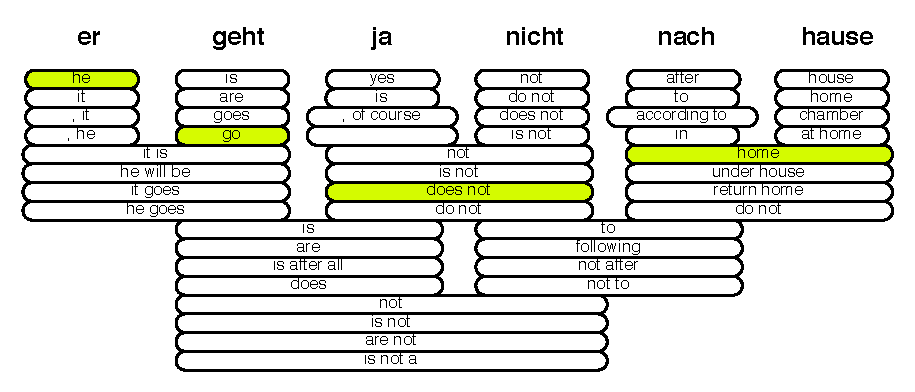
\includegraphics[scale=1.5]{translation-options-correct.pdf}
\end{center}  \vspace{-12mm}
\begin{itemize}
\item The machine translation decoder does not know the right answer\vspace{-4mm}
\begin{itemize}
\item picking the right translation options
\item arranging them in the right order \vspace{-6mm}
\end{itemize}
\item[$\rightarrow$] Search problem solved by heuristic beam search
\end{itemize}

%%%%%%%%%%%%%%%%%%%%%%%%%%%%%%%%%%%%%%%%%%%%%%%%%%%%%%%%%%%%%%%%%%%%%%%%%%%%%

\slide{Decoding: Precompute Translation Options}
\begin{center}
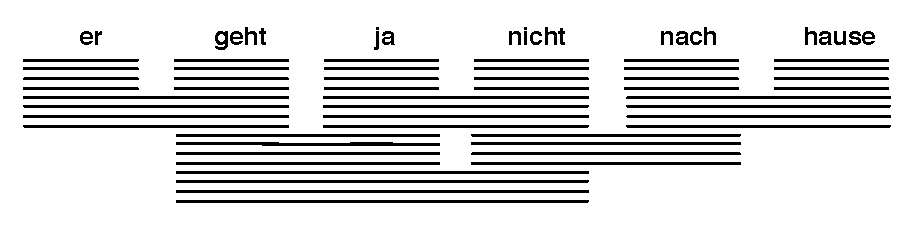
\includegraphics[scale=1.3]{decoding-step1.pdf}\\[69mm]
consult phrase translation table for all input phrases
\end{center}

%%%%%%%%%%%%%%%%%%%%%%%%%%%%%%%%%%%%%%%%%%%%%%%%%%%%%%%%%%%%%%%%%%%%%%%%%%%%

\slide{Decoding: Start with Initial Hypothesis}
\begin{center} 
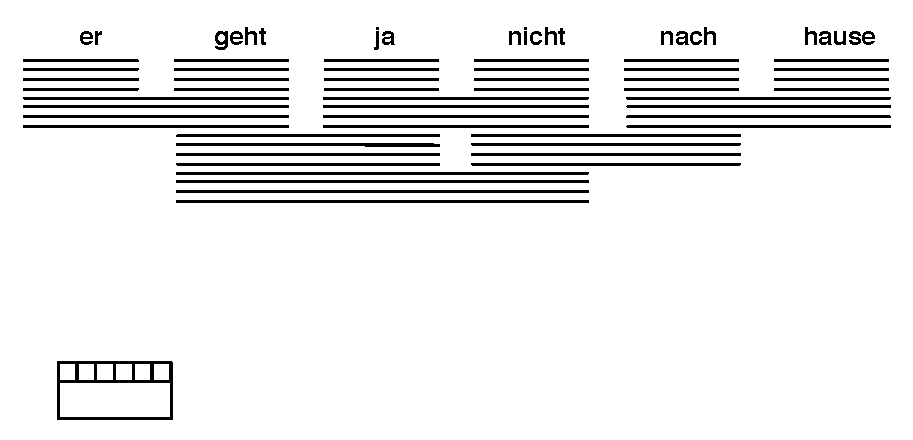
\includegraphics[scale=1.3]{decoding-step2.pdf}\\[22mm]
initial hypothesis: no input words covered, no output produced
\end{center}

%%%%%%%%%%%%%%%%%%%%%%%%%%%%%%%%%%%%%%%%%%%%%%%%%%%%%%%%%%%%%%%%%%%%%%%%%%%%

\slide{Decoding: Hypothesis Expansion}
\begin{center}
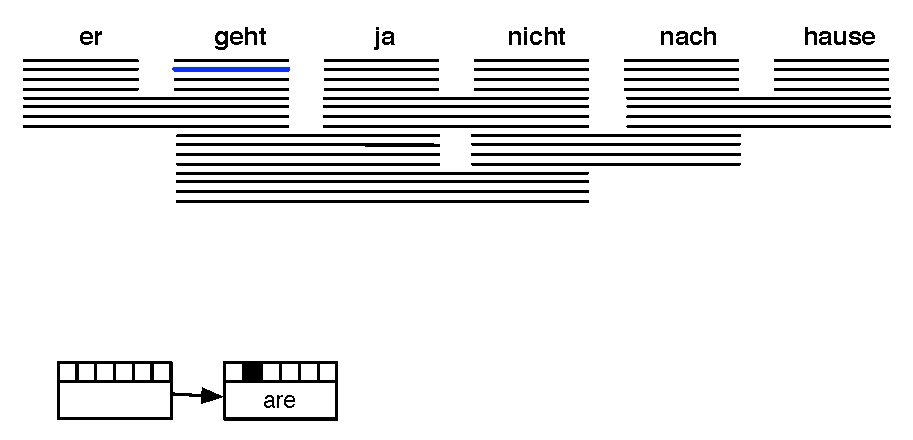
\includegraphics[scale=1.3]{decoding-step3.pdf}\\[22mm]
pick any translation option, create new hypothesis
\end{center} 

%%%%%%%%%%%%%%%%%%%%%%%%%%%%%%%%%%%%%%%%%%%%%%%%%%%%%%%%%%%%%%%%%%%%%%%%%%%%

\slide{Decoding: Hypothesis Expansion}
\begin{center} 
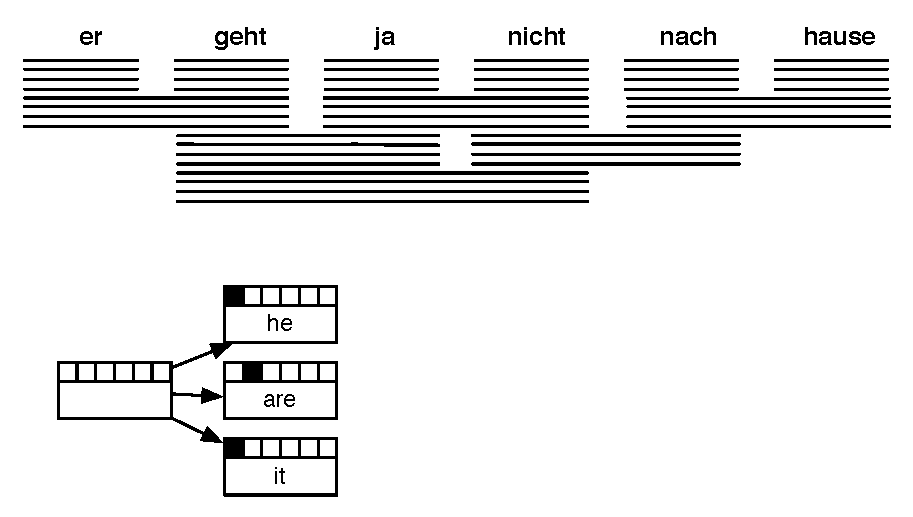
\includegraphics[scale=1.3]{decoding-step4.pdf}\\[5mm]
create hypotheses for all other translation options
\end{center}

%%%%%%%%%%%%%%%%%%%%%%%%%%%%%%%%%%%%%%%%%%%%%%%%%%%%%%%%%%%%%%%%%%%%%%%%%%%%

\slide{Decoding: Hypothesis Expansion}
\begin{center} 
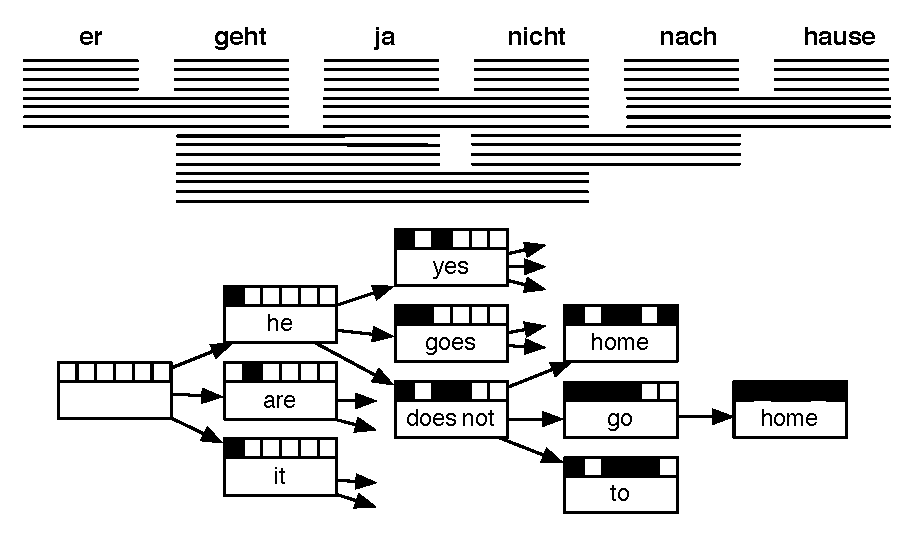
\includegraphics[scale=1.3]{decoding-step5.pdf}\\
also create hypotheses from created partial hypothesis
\end{center}

%%%%%%%%%%%%%%%%%%%%%%%%%%%%%%%%%%%%%%%%%%%%%%%%%%%%%%%%%%%%%%%%%%%%%%%%%%%%

\slide{Decoding: Find Best Path}
\begin{center}
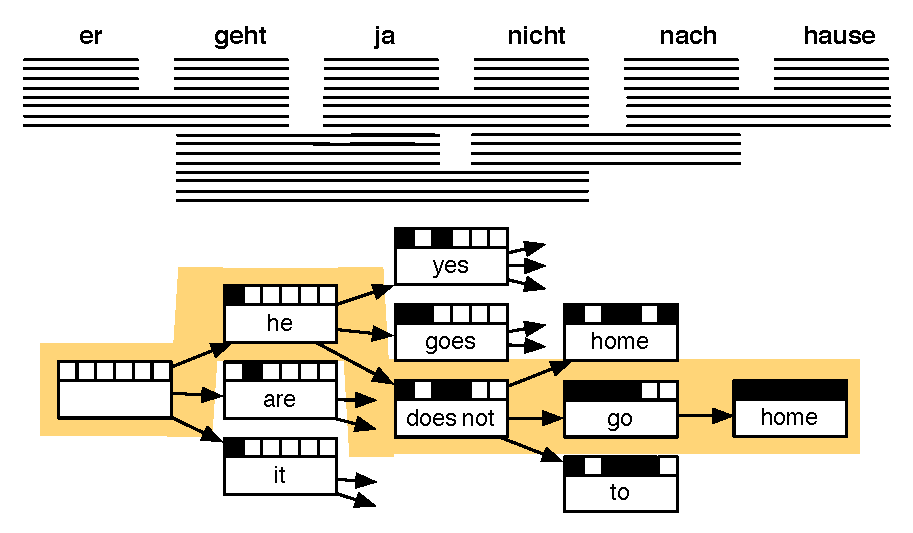
\includegraphics[scale=1.3]{decoding-step6.pdf}\\[1mm]
backtrack from highest scoring complete hypothesis
\end{center}

%%%%%%%%%%%%%%%%%%%%%%%%%%%%%%%%%%%%%%%%%%%%%%%%%%%%%%%%%%%%%%%%%%%%%%%%%%%%

\slide{Computational Complexity}
\begin{itemize}\vspace{35mm} \itemsep 5mm
\item The suggested process creates exponential number of hypothesis 
\item Reduction of search space: pruning
\item[$\rightarrow$] Decoder may not find the model-best translation
\end{itemize}

%%%%%%%%%%%%%%%%%%%%%%%%%%%%%%%%%%%%%%%%%%%%%%%%%%%%%%%%%%%%%%%%%%%%%%%%%%%%

\slide{Factored Represention}
\begin{itemize}
\item Factored represention of words 
\begin{center} \vspace{-8mm}
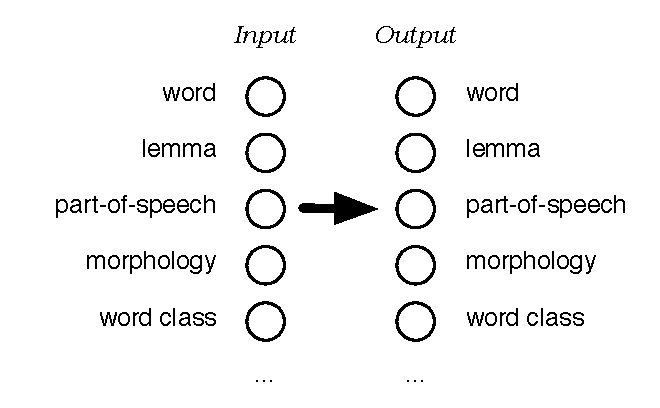
\includegraphics[width=155mm]{factors.pdf}
\end{center} \vspace{-22mm}
\item Goals  \vspace{-3mm}
\begin{itemize}
\item generalization, e.g. by translating lemmas, not surface forms
\item richer model, e.g. using syntax for reordering, language modeling)
\end{itemize}
\end{itemize}

%%%%%%%%%%%%%%%%%%%%%%%%%%%%%%%%%%%%%%%%%%%%%%%%%%%%%%%%%%%%%%%%%%%%%%%%%%%%

\slide{Factored Model}
\begin{center}
Example:\\
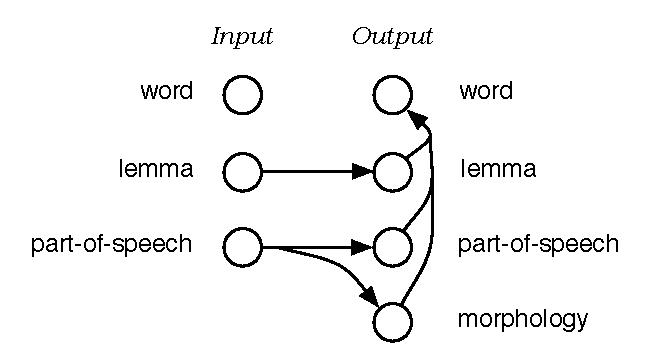
\includegraphics[scale=1.6]{factored-morphgen.pdf}\\
Decomposing the translation step\\
Translating lemma and morphological information more robust
\end{center}

%%%%%%%%%%%%%%%%%%%%%%%%%%%%%%%%%%%%%%%%%%%%%%%%%%%%%%%%%%%%%%%%%%%%%%%%%%%%

\slide{Syntax Models}
\vspace{5mm}
{\small
\begin{center}
\begin{tabular}{cc}
\textcolor{black}{\bf String to String} & \textcolor{black}{\bf String to Tree} \\
\example{John misses Mary}
& \example{John misses Mary}\\
$\Rightarrow$  Marie manque \`a Jean
& $\Rightarrow$ \hspace{-2cm} \Tree [.S [.NP \example{Marie} ] [.VP [.V \example{manque} ] [.PP [.P \example{\`a} ] [.NP \example{Jean} ]  ]  ]  ]\\[5mm]

\textcolor{black}{\bf Tree to String} & \textcolor{black}{\bf Tree to Tree} \\
\Tree [.S [.NP \example{John} ] [.VP [.V \example{misses} ] [.NP \example{Mary} ]  ]  ] 
&  \Tree [.S [.NP \example{John} ] [.VP [.V \example{misses} ] [.NP \example{Mary} ]  ]  ] \hspace{-1cm} $\Rightarrow$ \hspace{-2cm}\Tree [.S [.NP \example{Marie} ] [.VP [.V \example{manque} ] [.PP [.P \example{\`a} ] [.NP \example{Jean} ]  ]  ]  ] \\[-1cm]
$\Rightarrow$ \example{Marie manque \`a Jean}  	
& 
\end{tabular}
\end{center}
}

%%%%%%%%%%%%%%%%%%%%%%%%%%%%%%%%%%%%%%%%%%%%%%%%%%%%%%%%%%%%%%%%%%%%%%%%%%%%

\slide{Syntax Decoding}
\vspace{-31mm}
\begin{center}
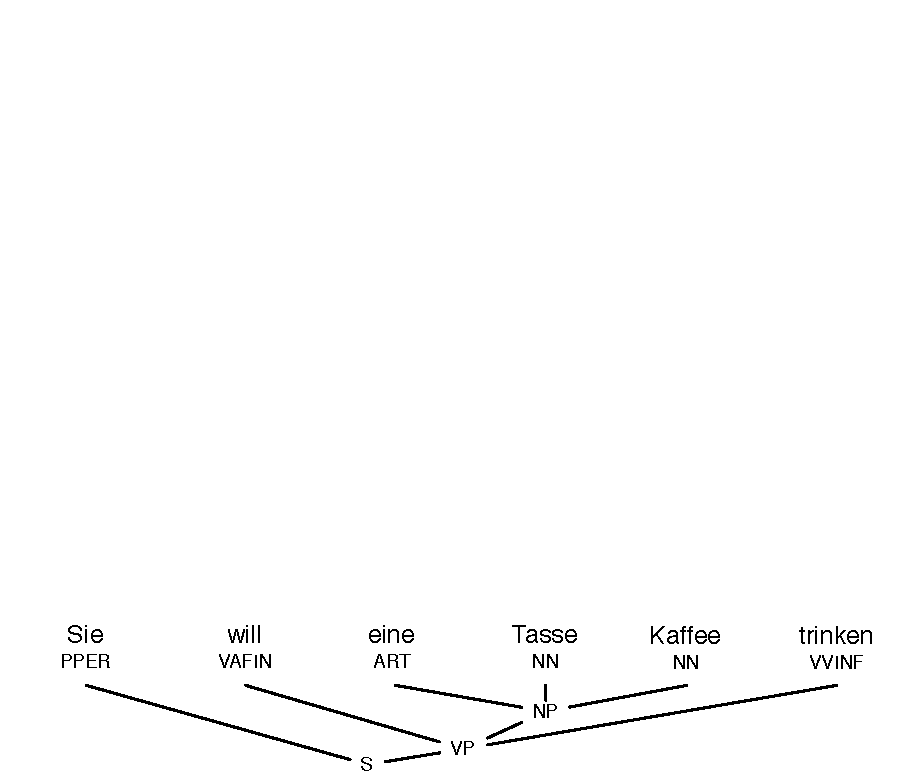
\includegraphics[scale=1.15]{chart-parsing0.pdf}
\end{center}

%%%%%%%%%%%%%%%%%%%%%%%%%%%%%%%%%%%%%%%%%%%%%%%%%%%%%%%%%%%%%%%%%%%%%%%%%%%%

\slide{Syntax Decoding}
\vspace{-31mm}
\begin{center}
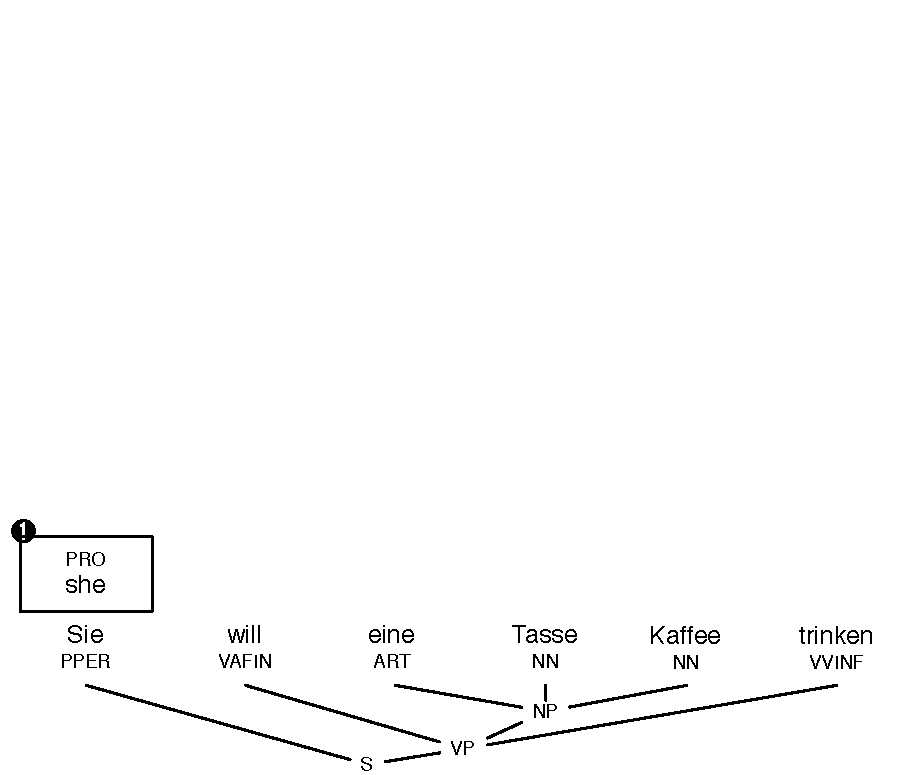
\includegraphics[scale=1.15]{chart-parsing1.pdf}
\end{center}

%%%%%%%%%%%%%%%%%%%%%%%%%%%%%%%%%%%%%%%%%%%%%%%%%%%%%%%%%%%%%%%%%%%%%%%%%%%%

\slide{Syntax Decoding}
\vspace{-31mm}
\begin{center}
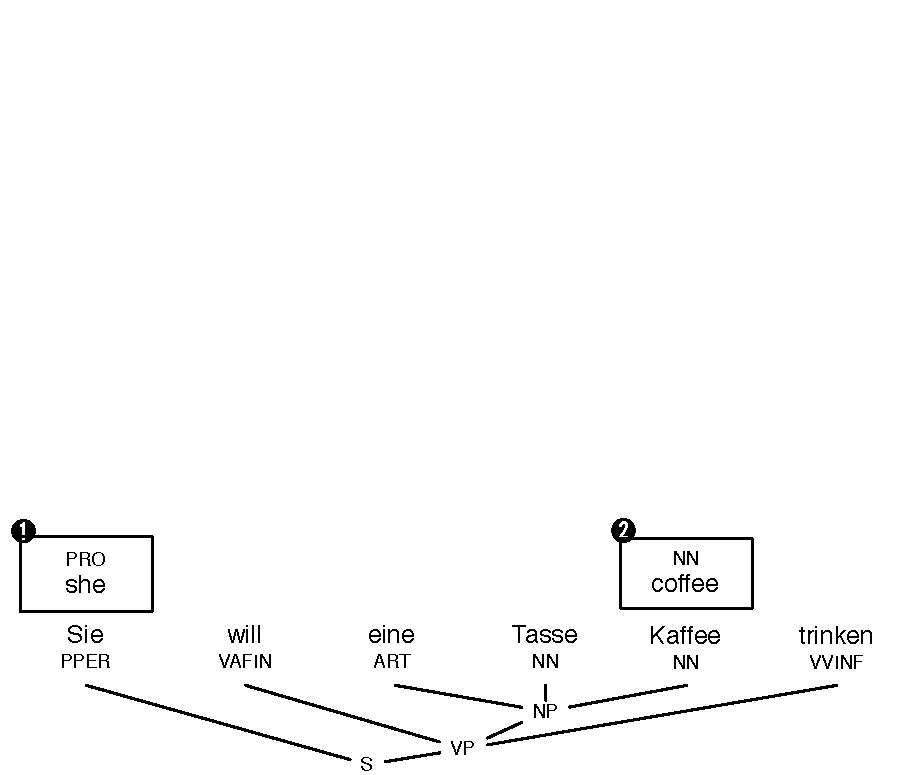
\includegraphics[scale=1.15]{chart-parsing2.pdf}
\end{center}

%%%%%%%%%%%%%%%%%%%%%%%%%%%%%%%%%%%%%%%%%%%%%%%%%%%%%%%%%%%%%%%%%%%%%%%%%%%%

\slide{Syntax Decoding}
\vspace{-31mm}
\begin{center}
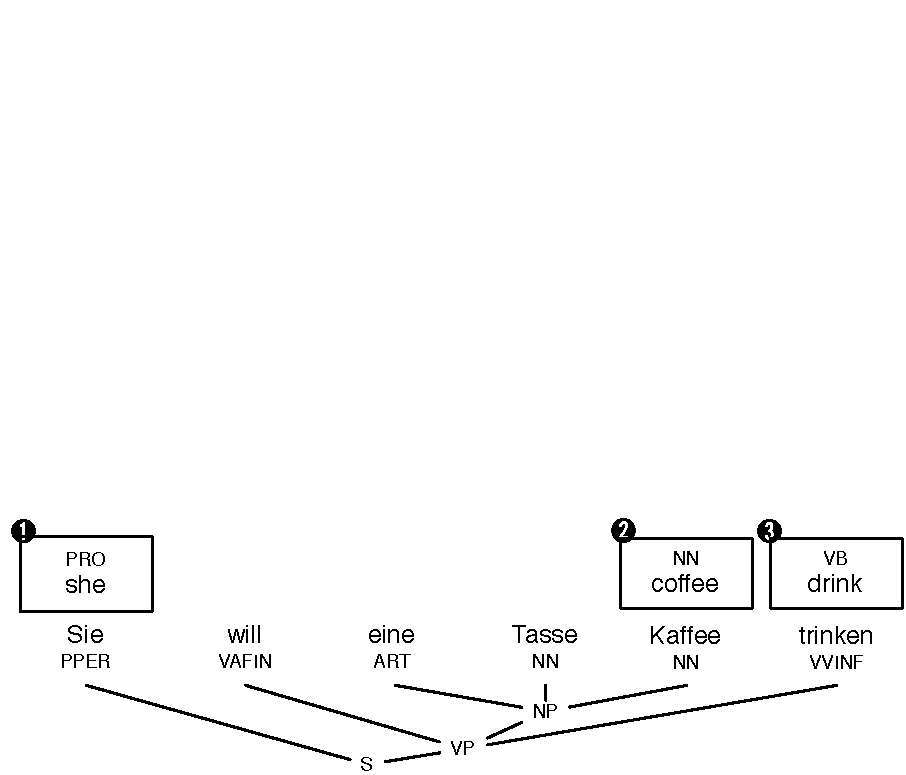
\includegraphics[scale=1.15]{chart-parsing3.pdf}
\end{center}

%%%%%%%%%%%%%%%%%%%%%%%%%%%%%%%%%%%%%%%%%%%%%%%%%%%%%%%%%%%%%%%%%%%%%%%%%%%%

\slide{Syntax Decoding}
\vspace{-31mm}
\begin{center}
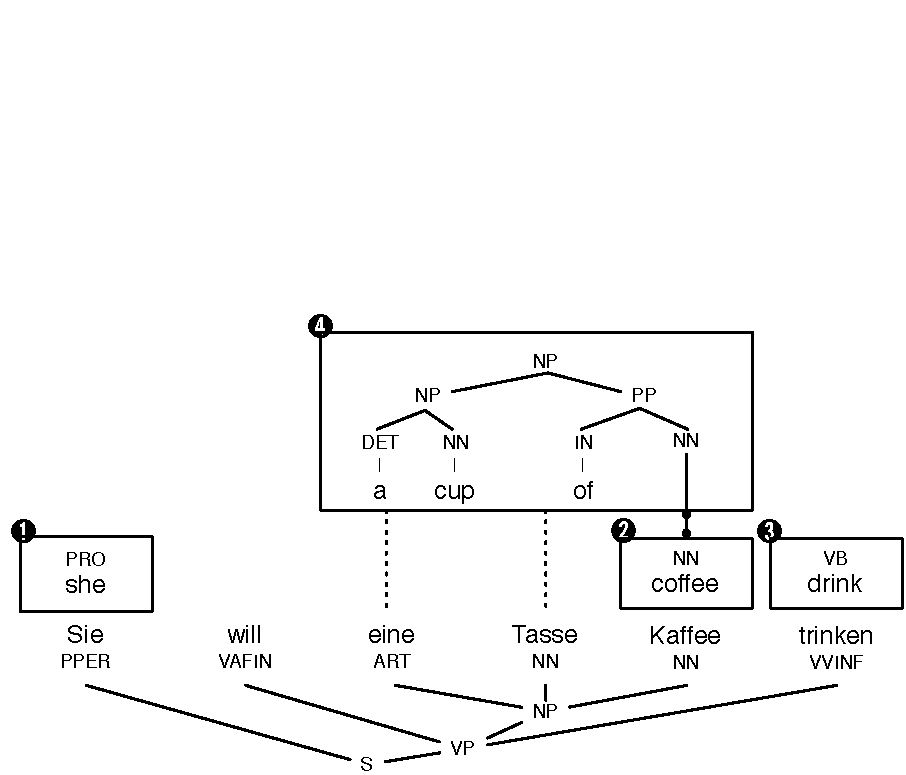
\includegraphics[scale=1.15]{chart-parsing4.pdf}
\end{center}

%%%%%%%%%%%%%%%%%%%%%%%%%%%%%%%%%%%%%%%%%%%%%%%%%%%%%%%%%%%%%%%%%%%%%%%%%%%%

\slide{Syntax Decoding}
\vspace{-31mm}
\begin{center}
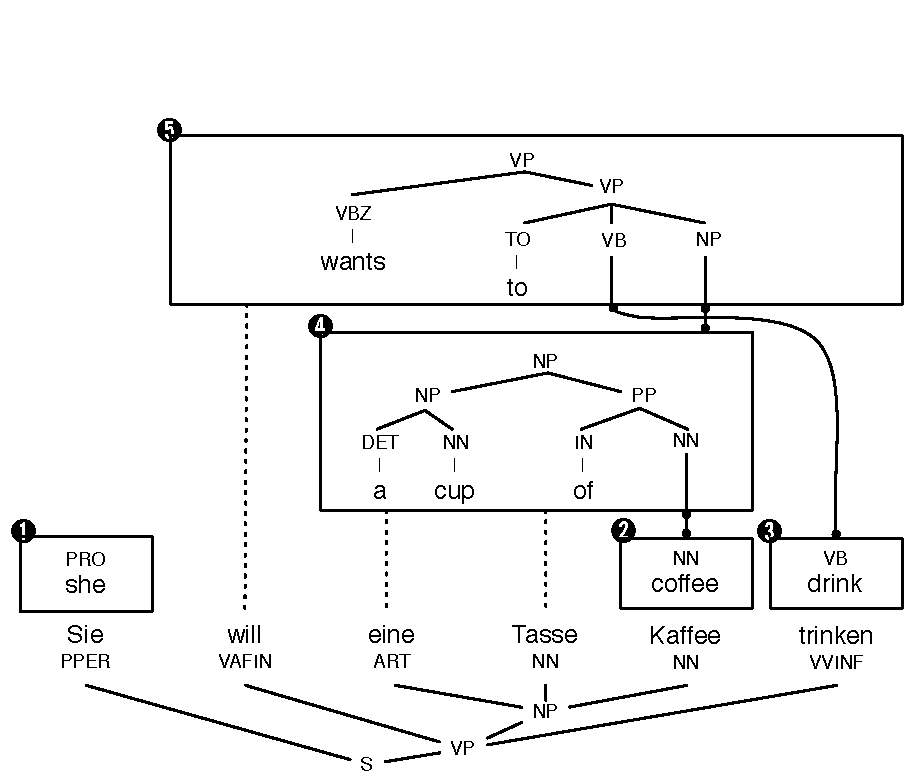
\includegraphics[scale=1.15]{chart-parsing5.pdf}
\end{center}

%%%%%%%%%%%%%%%%%%%%%%%%%%%%%%%%%%%%%%%%%%%%%%%%%%%%%%%%%%%%%%%%%%%%%%%%%%%%

\slide{Syntax Decoding}
\vspace{-31mm}
\begin{center}
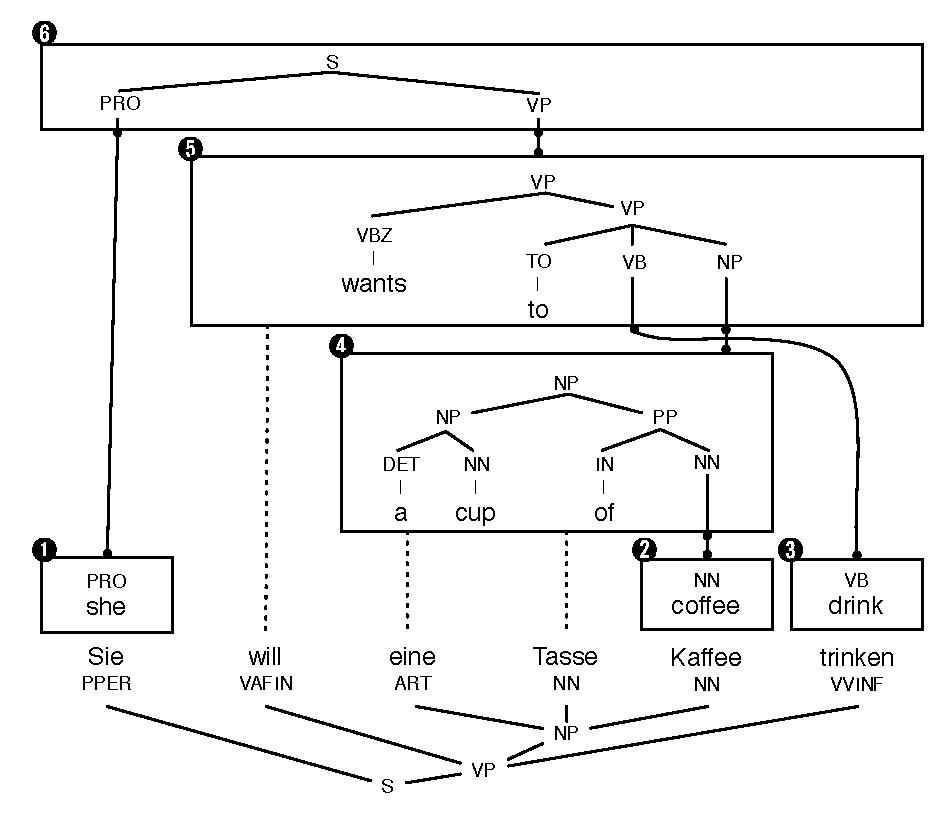
\includegraphics[scale=1.15]{chart-parsing.pdf}
\end{center}

%%%%%%%%%%%%%%%%%%%%%%%%%%%%%%%%%%%%%%%%%%%%%%%%%%%%%%%%%%%%%%%%%%%%%%%%%%%%


%%%%%%%%%%%%%%%%%%%%%%%%%%%%%%%%%%%%%%%%%%%%%%%%%%%%%%%%%%%%%%%%%%%%%%%%%%%%
\slide{}
\vspace{50mm}
\begin{center}
\Huge \bf Advanced Features
\end{center}


\slide{Advanced Features}
\small
\vspace{-5mm}
\textcolor{darkgrey}{
\begin{itemize} \itemsep -1mm
\item \currenttopic{How do I get started?}
\item {Experiment Management System}
\item {Faster Decoding}
\item {Data and domain adaptation}
\item {Instructions to decoder}
\item {Input formats}
\item {Output formats}
\end{itemize}
}

%%%%%%%%%%%%%%%%%%%%%%%%%%%%%%%%%%%%%%%%%%%%%%%%%%%%%%%%%%%%%%%%%%%%%%%%%%%%

\slide{How do I get started?}
\normalsize
\begin{itemize} \itemsep -1mm

\item{Collect your data}
  \begin{itemize}
  \item Parallel data 
  \item Translation memories
  \item Open-sourced data, eg. Europarl, UN, TAUS Data Association
  \item Monolingual data
  \end{itemize}
\item{Set up Moses}
  \begin{itemize}
  \item Download source code for Moses, GIZA++, MGIZA
  \item Compile, install
  \item More info:
        http://www.statmt.org/moses/
  \item Prepackaged Moses:
        Precision Tools, MacPorts, Debian packages, M4Loc
  \end{itemize}
\end{itemize}

%%%%%%%%%%%%%%%%%%%%%%%%%%%%%%%%%%%%%%%%%%%%%%%%%%%%%%%%%%%%%%%%%%%%%%%%%%%%

\slide{How do I get started?}
{\small

\begin{center}
\textcolor{red}{Execute a lot of scripts} \\
\begin{SaveVerbatim}{myverb}
tokenize < corpus.en > corpus.en.tok
lowercase < corpus.en.tok > corpus.en.lc
...
mert.perl ....
moses ...
mteval-v13.pl ...
\end{SaveVerbatim}
\colorbox{gray}{\BUseVerbatim{myverb}}

\vspace{10mm}
\textcolor{red}{Change a part of the process, execute everything again} \\
\begin{SaveVerbatim}{myverb}
tokenize < corpus.en > corpus.en.tok
lowercase < corpus.en.tok > corpus.en.lc
...
mert.perl ....
moses ...
mteval-v13.pl ...
\end{SaveVerbatim}
\colorbox{gray}{\BUseVerbatim{myverb}}
\end{center}
}

%%%%%%%%%%%%%%%%%%%%%%%%%%%%%%%%%%%%%%%%%%%%%%%%%%%%%%%%%%%%%%%%%%%%%%%%%%%%

% \slide{How do I get started?}
% 
% \begin{itemize} \itemsep -1mm
% 
% \item{Use the {\bf Experiment Management System (EMS)} } 
%   \begin{itemize}
%   \item Automate entire process
%   \item Support for multi-core servers. And Sun Grid Engines (SGE)
%   \item Reuse existing alignments or models when running multiple, similar experiments
%   \item Example config files available in Moses
%   \item Disadvantage --- not all features are implemented
%   \end{itemize}
% 
% \end{itemize}

%%%%%%%%%%%%%%%%%%%%%%%%%%%%%%%%%%%%%%%%%%%%%%%%%%%%%%%%%%%%%%%%%%%%%%%%%%%%


\slide{Advanced Features}
\vspace{-5mm}
\textcolor{darkgrey}{
\small
\begin{itemize} \itemsep -1mm
\item {How do I get started?}
\item \currenttopic{Experiment Management System}
\item {Faster Decoding}
\item {Data and domain adaptation}
\item {Instructions to decoder}
\item {Input formats}
\item {Output formats}
\end{itemize}
}

%%%%%%%%%%%%%%%%%%%%%%%%%%%%%%%%%%%%%%%%%%%%%%%%%%%%%%%%%%%%%%%%%%%%%%%%%%%%
\slide{Experiment Management System}
\begin{itemize} \itemsep -1mm
\item One configuration file for all settings: record of all experimental details
\item Scheduler of individual steps in pipeline
\begin{itemize}
\item automatically keeps track of dependencies
\item runs on single machine, multi-core machine, GridEngine cluster
\item parallel execution 
\item crash detection
\item automatic re-use of prior results
\end{itemize}
\item Fast to use
\begin{itemize}
\item set up a new experiment in minutes
\item set up a variation of an experiment in seconds
\end{itemize}

\item Disadvantage --- not all Moses features are integrated

\end{itemize}

%%%%%%%%%%%%%%%%%%%%%%%%%%%%%%%%%%%%%%%%%%%%%%%%%%%%%%%%%%%%%%%%%%%%%%%%%%%%

\slide{}
\begin{center} \vspace{-5mm}
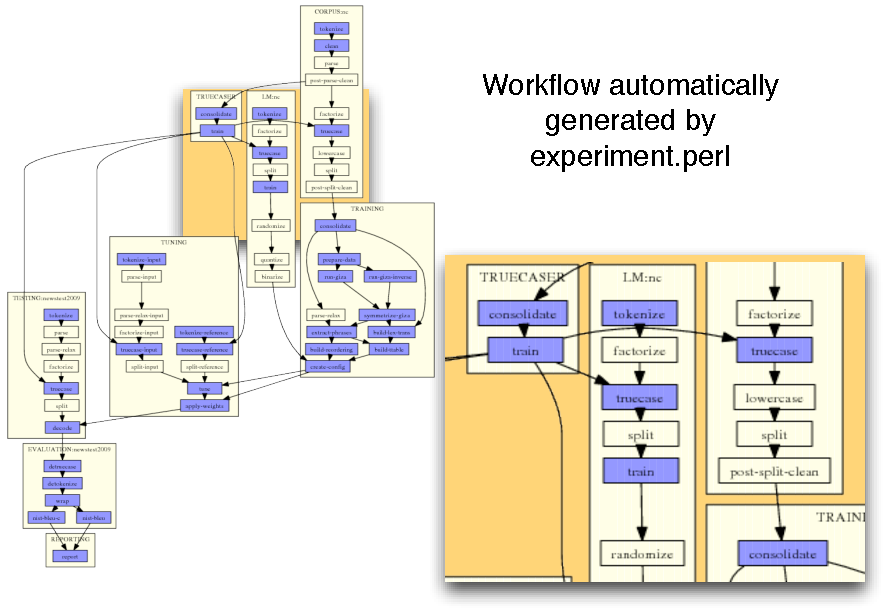
\includegraphics[scale=1.41]{ems-agenda-composite.pdf}
\end{center}

%%%%%%%%%%%%%%%%%%%%%%%%%%%%%%%%%%%%%%%%%%%%%%%%%%%%%%%%%%%%%%%%%%%%%%%%%%%%

\slide{How does it work?}
\vspace{20mm}
\begin{itemize}
\item Write a configuration file
(typically by adapting an existing file)
\vspace{5mm}
\item Test:
\vspace{-10mm}
\begin{center}
\littlecode{\normalsize experiment.perl -config config}
\end{center}
\vspace{5mm}
\item Execute:
\vspace{-10mm}
\begin{center}
\littlecode{\normalsize experiment.perl -config config -exec}
\end{center}
\end{itemize}

%%%%%%%%%%%%%%%%%%%%%%%%%%%%%%%%%%%%%%%%%%%%%%%%%%%%%%%%%%%%%%%%%%%%%%%%%%%%

\slide{Web Interface}
\begin{center}
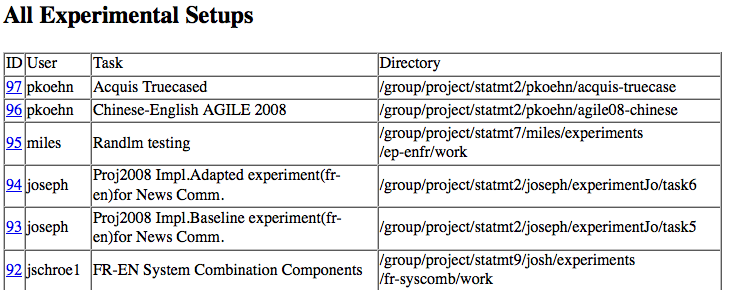
\includegraphics[scale=1]{web-interface-experiments.png}\\[5mm]
List of experiments
\end{center}

%%%%%%%%%%%%%%%%%%%%%%%%%%%%%%%%%%%%%%%%%%%%%%%%%%%%%%%%%%%%%%%%%%%%%%%%%%%%

\slide{List of Runs}
\begin{center}\vspace{-9mm}
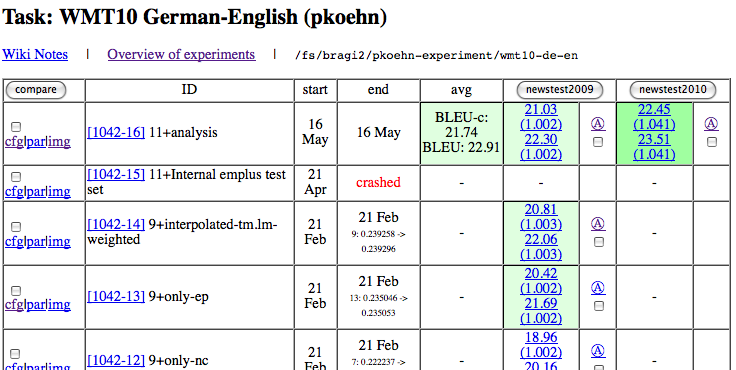
\includegraphics[scale=1]{web-interface-runs}
\end{center}

%%%%%%%%%%%%%%%%%%%%%%%%%%%%%%%%%%%%%%%%%%%%%%%%%%%%%%%%%%%%%%%%%%%%%%%%%%%%

\slide{Analysis: Basic Statistics}
\begin{center}
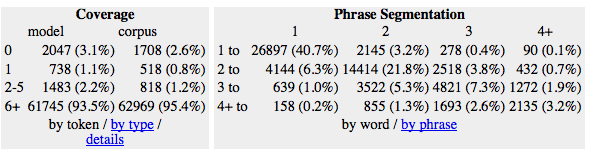
\includegraphics[scale=1]{analysis-stats.png}
\end{center}
\begin{itemize}
\item Basic statistics
\begin{itemize}
\item n-gram precision
\item evaluation metrics
\item coverage of the input in corpus and translation model
\item phrase segmentations used
\end{itemize}
\end{itemize}

%%%%%%%%%%%%%%%%%%%%%%%%%%%%%%%%%%%%%%%%%%%%%%%%%%%%%%%%%%%%%%%%%%%%%%%%%%%%

\slide{Analysis: Unknown Words}
\begin{center}
grouped by count in test set\\[5mm]
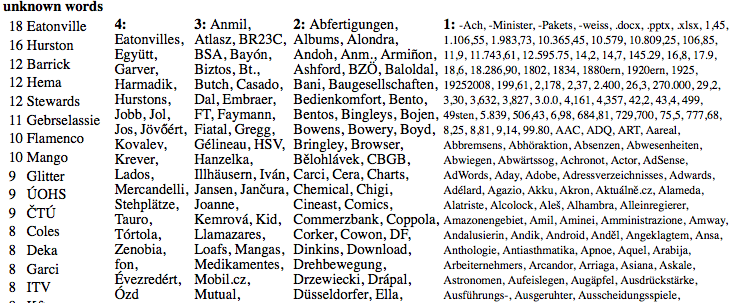
\includegraphics[scale=1]{analysis-unknown.png}
\end{center}

%%%%%%%%%%%%%%%%%%%%%%%%%%%%%%%%%%%%%%%%%%%%%%%%%%%%%%%%%%%%%%%%%%%%%%%%%%%%

\slide{Analysis: Output Annotation}
\vspace{30mm}
\begin{center}
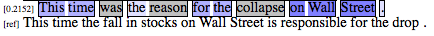
\includegraphics[scale=1.5]{analysis-bleu.png}\\[20mm]
Color highlighting to indicate n-gram overlap with reference translation\\[5mm]
darker bleu = word is part of larger n-gram match
\end{center}

%%%%%%%%%%%%%%%%%%%%%%%%%%%%%%%%%%%%%%%%%%%%%%%%%%%%%%%%%%%%%%%%%%%%%%%%%%%%

\slide{Analysis: Input Annotation}
\vspace{10mm}
\begin{center}
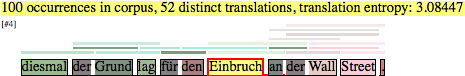
\includegraphics[scale=1.5]{analysis-coverage.png}\\[20mm]
\end{center}
\begin{itemize}
\item For each word and phrase, color coding and stats on
\begin{itemize}
\item number of occurrences in training corpus
\item number of distinct translations in translation model
\item entropy of conditional translation probability distribution $\phi(e|f)$ (normalized)
\end{itemize}
\end{itemize}

%%%%%%%%%%%%%%%%%%%%%%%%%%%%%%%%%%%%%%%%%%%%%%%%%%%%%%%%%%%%%%%%%%%%%%%%%%%%

\slide{Analysis: Bilingual Concordancer}
\vspace{-5mm}
\begin{center}
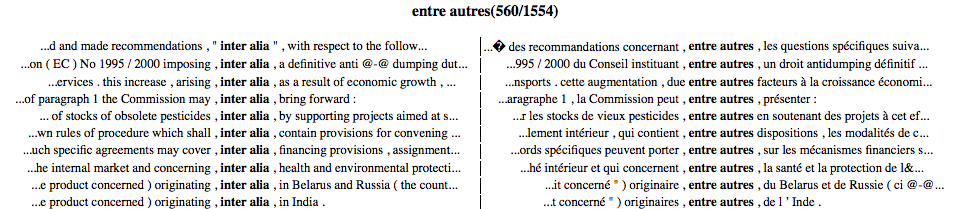
\includegraphics[scale=0.75]{biconcor1.png}\\[5mm]

\includegraphics[scale=0.75]{biconcor2.png}\\
translation of input phrase in training data context
\end{center}

%%%%%%%%%%%%%%%%%%%%%%%%%%%%%%%%%%%%%%%%%%%%%%%%%%%%%%%%%%%%%%%%%%%%%%%%%%%%

\slide{Analysis: Alignment}
\vspace{30mm}
\begin{center}
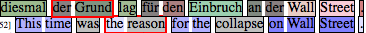
\includegraphics[scale=1.5]{analysis-alignment.png}\\[10mm]
Phrase alignment of the decoding process\\[5mm]
(red border, interactive)
\end{center}

%%%%%%%%%%%%%%%%%%%%%%%%%%%%%%%%%%%%%%%%%%%%%%%%%%%%%%%%%%%%%%%%%%%%%%%%%%%%

\slide{Analysis: Tree Alignment}
\vspace{15mm}
\begin{center}
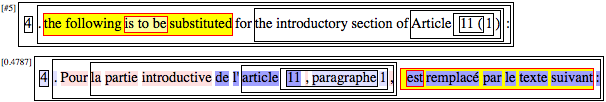
\includegraphics[scale=1.2]{analysis-tree-alignment.png}\\[10mm]
Uses nested boxes to indicate tree structure\\[3mm]
(red border, yellow shaded spans in focus, interactive)\\[3mm]
for syntax model, non-terminals are also shown
\end{center}



%%%%%%%%%%%%%%%%%%%%%%%%%%%%%%%%%%%%%%%%%%%%%%%%%%%%%%%%%%%%%%%%%%%%%%%%%%%%

\slide{}
\vspace{-2.5cm}
\begin{center}
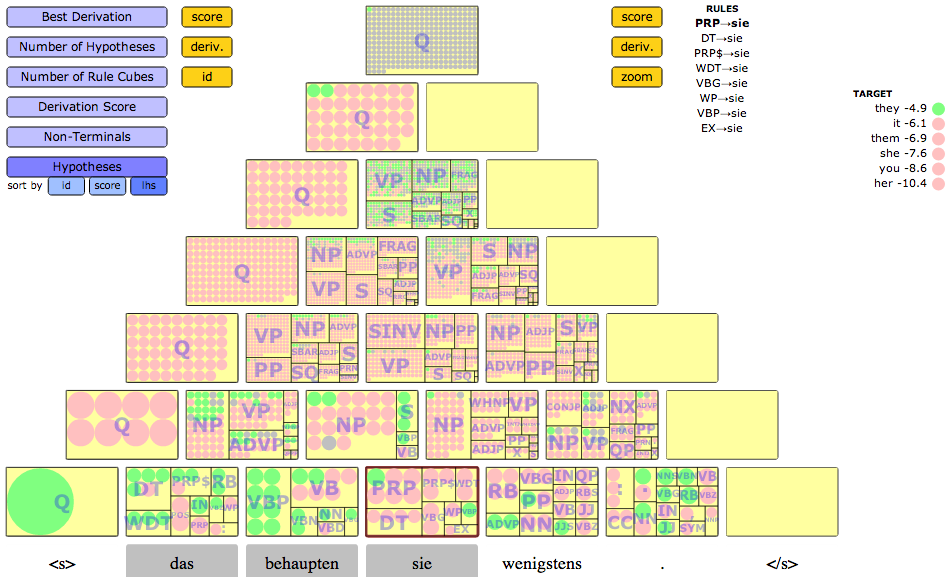
\includegraphics[width=26cm]{ems-syntax-viz.png}
\end{center}

%%%%%%%%%%%%%%%%%%%%%%%%%%%%%%%%%%%%%%%%%%%%%%%%%%%%%%%%%%%%%%%%%%%%%%%%%%%%

\slide{Analysis: Comparison of 2 Runs}
\begin{center}
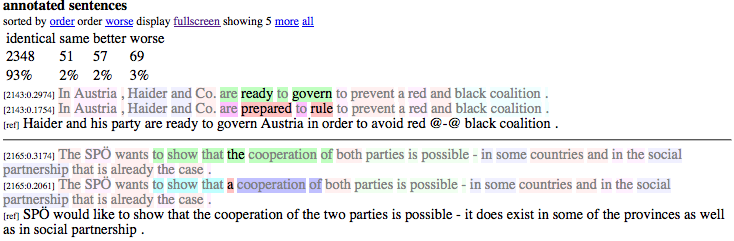
\includegraphics[scale=1]{analysis-comparison.png}\\[10mm]
Different words are highlighted\\[3mm]
sortable by most improvement, deterioration
\end{center}

%%%%%%%%%%%%%%%%%%%%%%%%%%%%%%%%%%%%%%%%%%%%%%%%%%%%%%%%%%%%%%%%%%%%%%%%%%%%

\slide{Advanced Features}
\vspace{-5mm}
\textcolor{darkgrey}{
\small
\begin{itemize} \itemsep -1mm
\item {How do I get started?}
\item {Experiment Management System}
\item {Faster Decoding}
\item {Data and domain adaptation}
\item {Instructions to decoder}
\item {Input formats}
\item {Output formats}
\end{itemize}
}

\slide{Advanced Features}
\vspace{-5mm}
\textcolor{darkgrey}{
\small
\begin{itemize} \itemsep -1mm
\item {How do I get started?}
\item {Experiment Management System}
\item \currenttopic{Faster Decoding}
\item {Data and domain adaptation}
\item {Instructions to decoder}
\item {Input formats}
\item {Output formats}
\end{itemize}
}

%%%%%%%%%%%%%%%%%%%%%%%%%%%%%%%%%%%%%%%%%%%%%%%%%%%%%%%%%%%%%%%%%%%%%%%%%%%%

\slide{Advanced Features}
\vspace{-5mm}
\textcolor{darkgrey}{
\begin{itemize} \itemsep -1mm
\item {How do I get started?}
\item {Experiment Management System}
\item \currenttopic{Faster Decoding}
  \begin{itemize}
  \item Speed vs. Memory
  \item Speed vs. Quality
  \end{itemize}
\end{itemize}
...
}

%%%%%%%%%%%%%%%%%%%%%%%%%%%%%%%%%%%%%%%%%%%%%%%%%%%%%%%%%%%%%%%%%%%%%%%%%%%%

\slide{Advanced Features}
\vspace{-5mm}
\textcolor{darkgrey}{
\begin{itemize} \itemsep -1mm
\item {How do I get started?}
\item {Experiment Management System}
\item {Faster Decoding}
  \begin{itemize}
  \item Speed vs. Memory
  \item Speed vs. Quality
  \end{itemize}
\end{itemize}
...
}

%%%%%%%%%%%%%%%%%%%%%%%%%%%%%%%%%%%%%%%%%%%%%%%%%%%%%%%%%%%%%%%%%%%%%%%%%%%%

\slide{Advanced Features}
\vspace{-5mm}
\textcolor{darkgrey}{
\begin{itemize} \itemsep -1mm
\item {How do I get started?}
\item {Experiment Management System}
\item {Faster Training}
\item {Faster Decoding}
  \begin{itemize}
  \item \currenttopic{Speed vs. Memory}
  \item Speed vs. Quality
  \end{itemize}
\end{itemize}
...
}

%%%%%%%%%%%%%%%%%%%%%%%%%%%%%%%%%%%%%%%%%%%%%%%%%%%%%%%%%%%%%%%%%%%%%%%%%%%%

%\slide{Speed vs. Memory Use}
%\begin{center} 
%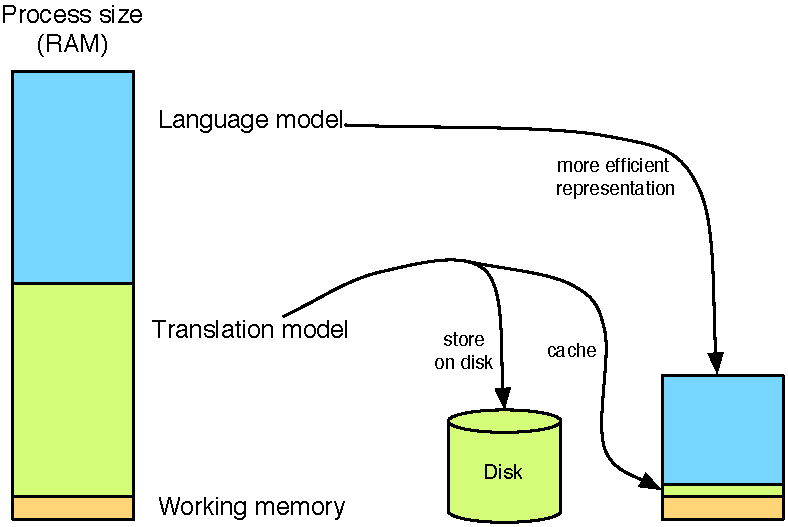
\includegraphics[scale=1.4]{less-memory.pdf}
%\end{center}

%%%%%%%%%%%%%%%%%%%%%%%%%%%%%%%%%%%%%%%%%%%%%%%%%%%%%%%%%%%%%%%%%%%%%%%%%%%%

\slide{Speed vs. Memory Use}
\begin{tabular}{p{10cm}c}
\vspace{-11cm}
Typical Europarl file sizes:
\begin{itemize} \itemsep -1mm
  \item Language model \vspace{-3mm}
	\begin{itemize}
  	\item  170 MB (trigram)
	\item 412 MB (5-gram)
	\end{itemize}
  \item Phrase table \vspace{-3mm}
	\begin{itemize}
  	\item  11GB
	\end{itemize}
  \item Lexicalized reordering \vspace{-3mm}
	\begin{itemize}
  	\item  9.4GB
	\end{itemize}
   \item[$\rightarrow$] total = 20.8 GB
\end{itemize}
&
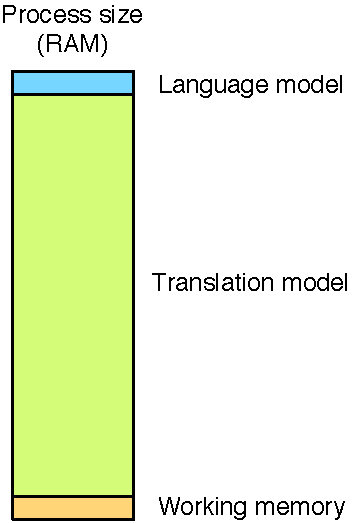
\includegraphics[scale=1.4]{less-memory-europarl.pdf}
\end{tabular}

%%%%%%%%%%%%%%%%%%%%%%%%%%%%%%%%%%%%%%%%%%%%%%%%%%%%%%%%%%%%%%%%%%%%%%%%%%%%

\slide{Speed vs. Memory Use}
\vspace{10mm}
\begin{tabular}{p{13cm}c}
\vspace{-7cm}
\begin{itemize}
\item Load into memory
	\begin{itemize}
	\item long load time
	\item large memory usage
	\item fast decoding
	\end{itemize}
\end{itemize}
& 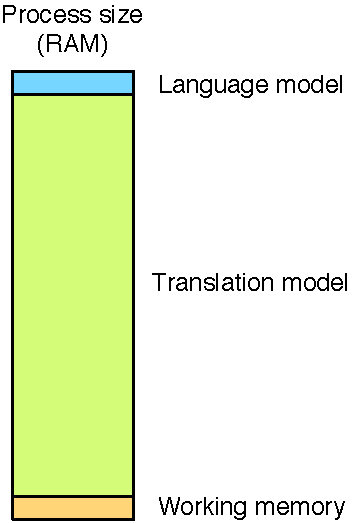
\includegraphics[scale=0.8]{less-memory-europarl.pdf} \\[1cm]
\vspace{-4.5cm}
\begin{itemize}
\item Load-on-demand
	\begin{itemize}
  	\item store indexed model on disk
	\item binary format
	\item minimal start-up time, memory usage
	\item slower decoding
	\end{itemize}
\end{itemize}
&  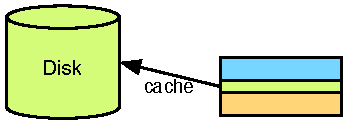
\includegraphics[scale=0.8]{less-memory-europarl-on-disk.pdf}
\end{tabular}

%%%%%%%%%%%%%%%%%%%%%%%%%%%%%%%%%%%%%%%%%%%%%%%%%%%%%%%%%%%%%%%%%%%%%%%%%%%%


\slide{New: Compact Phrase Table}
\begin{itemize}
\item Memory-efficient data structure
\begin{itemize}
\item phrase table 6--7 times smaller than on-disk binary table
\item lexical reordering table 12--15 times smaller than on-disk binary table
\end{itemize}
\item Stored in RAM
\item May be memory mapped
\end{itemize}

%%%%%%%%%%%%%%%%%%%%%%%%%%%%%%%%%%%%%%%%%%%%%%%%%%%%%%%%%%%%%%%%%%%%%%%%%%%%

\slide{IRSTLM}
\vspace{20mm}
\begin{itemize}
\item Developed by FBK-irst, Trento, Italy
\item Create a binary format which can be read from disk as needed
	\begin{itemize}
	\item reduces memory but slower decoding 
	\end{itemize}
\item Quantization of probabilities
	\begin{itemize}
	\item reduces memory but lose accuracy
	\item probability stored in 1 byte instead of 4 bytes
	\end{itemize}
\end{itemize}

%%%%%%%%%%%%%%%%%%%%%%%%%%%%%%%%%%%%%%%%%%%%%%%%%%%%%%%%%%%%%%%%%%%%%%%%%%%%

\slide{KENLM}
\vspace{10mm}
\begin{itemize}
\item Developed by Kenneth Heafield (CMU / Edinburgh / Stanford)
\item Fastest and smallest language model implementation
\end{itemize}

%%%%%%%%%%%%%%%%%%%%%%%%%%%%%%%%%%%%%%%%%%%%%%%%%%%%%%%%%%%%%%%%%%%%%%%%%%%%

\slide{Advanced Features}
\vspace{-5mm}
\textcolor{darkgrey}{
\begin{itemize} \itemsep -1mm
\item {How do I get started?}
\item {Experiment Management System}
\item {Faster Decoding}
  \begin{itemize}
  \item {Speed vs. Memory}
  \item \currenttopic{Speed vs. Quality}
  \end{itemize}
\end{itemize}
...
}


%%%%%%%%%%%%%%%%%%%%%%%%%%%%%%%%%%%%%%%%%%%%%%%%%%%%%%%%%%%%%%%%%%%%%%%%%%%%

\slide{Speed vs. Quality}
\vspace{5mm}
\begin{center} 
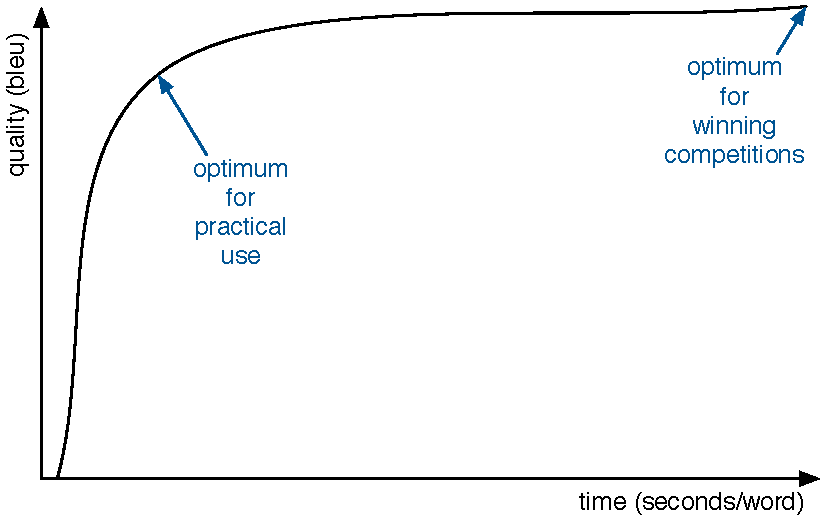
\includegraphics[scale=1.4]{quality-vs-speed.pdf}\vspace{-20mm}
\end{center}

%%%%%%%%%%%%%%%%%%%%%%%%%%%%%%%%%%%%%%%%%%%%%%%%%%%%%%%%%%%%%%%%%%%%%%%%%%%%

\slide{Speed vs. Quality}
\begin{center} 
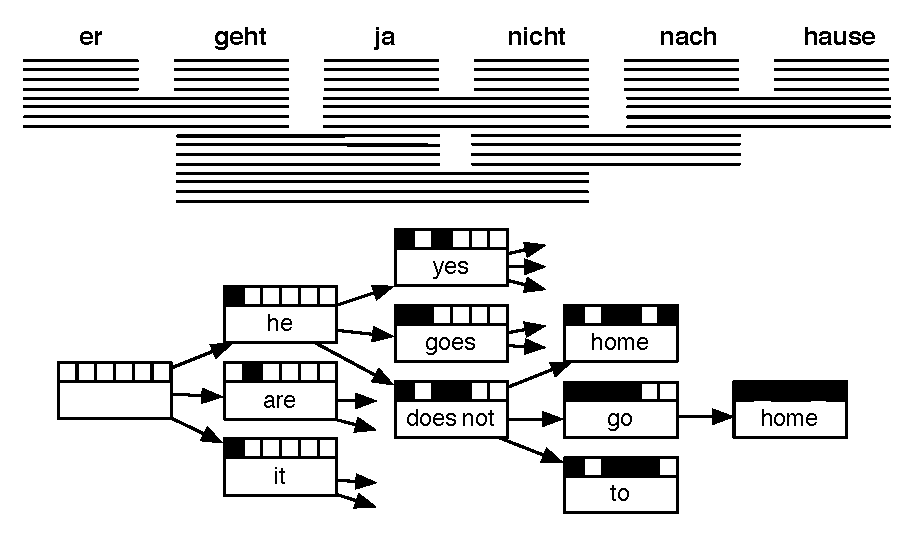
\includegraphics[scale=0.95]{decoding-step5.pdf}
\end{center}
\begin{itemize} \itemsep -1mm
\item Decoder search creates very large number of partial translations ("hypotheses")
\item Decoding time $\sim$ number of hypotheses created
\item Translation quality $\sim$ number of hypothesis created
\end{itemize}

%%%%%%%%%%%%%%%%%%%%%%%%%%%%%%%%%%%%%%%%%%%%%%%%%%%%%%%%%%%%%%%%%%%%%%%%%%%%

\slide{Hypothesis Stacks}
\begin{center} 
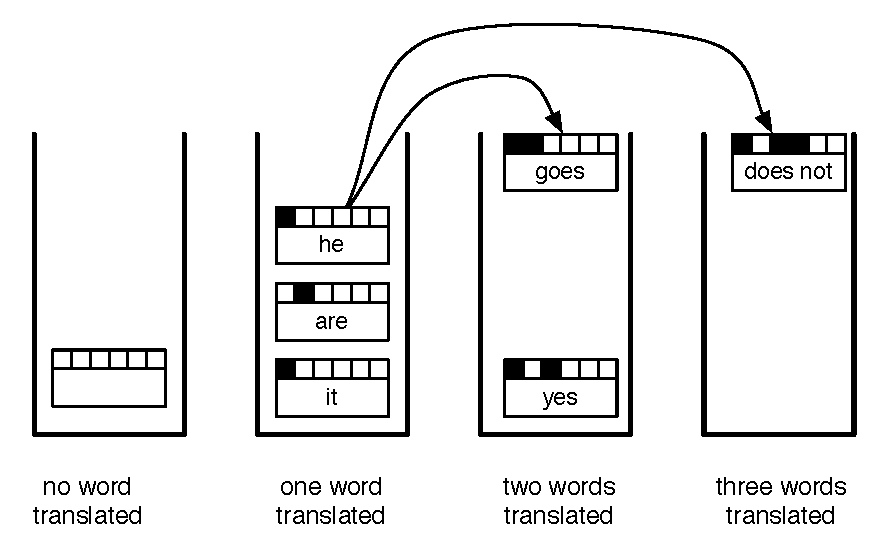
\includegraphics[scale=1]{hypothesis-stacks-fw.pdf}
\end{center}
\vspace{-2mm}
\begin{itemize} \itemsep -2mm
\item Phrase-based: One stack per number of input words covered
\item Number of hypothesis created = \\
sentence length $\times$ stack size $\times$ applicable translation options
\end{itemize}

\slide{Advanced Features}
\vspace{-5mm}
\textcolor{darkgrey}{
\begin{itemize} \itemsep -1mm
\item {How do I get started?}
\item {Experiment Management System}
\item {Faster Decoding}
\item {Data and domain adaptation}
\item {Instructions to decoder}
\item {Input formats}
\item {Output formats}
\end{itemize}
}

%%%%%%%%%%%%%%%%%%%%%%%%%%%%%%%%%%%%%%%%%%%%%%%%%%%%%%%%%%%%%%%%%%%%%%%%%%%%

\slide{Advanced Features}
\normalsize
\vspace{-5mm}
\textcolor{darkgrey}{
\small
\begin{itemize} \itemsep -1mm
\item {How do I get started?}
\item {Experiment Management System}
\item {Faster Decoding}
\item \currenttopic{Data and domain adaptation}
  \begin{itemize}\vspace{-4mm}
  \item Train everything together
  \item Secondary phrase table
\item Domain indicator features
\item Interpolated language models
  \item TM-MT integration
  \end{itemize}
\end{itemize}
}


%%%%%%%%%%%%%%%%%%%%%%%%%%%%%%%%%%%%%%%%%%%%%%%%%%%%%%%%%%%%%%%%%%%%%%%%%%%%

\slide{Data}
\vspace{15mm}
\begin{itemize}
\item Parallel corpora $\rightarrow$ translation model
\begin{itemize}
\item sentence-aligned translated texts
\item translation memories are parallel corpora
\item dictionaries are parallel corpora
\end{itemize}
\item Monolingual corpora $\rightarrow$ language model
\begin{itemize}
\item text in the target language
\item billions of words easy to handle
\end{itemize}
\end{itemize}

%%%%%%%%%%%%%%%%%%%%%%%%%%%%%%%%%%%%%%%%%%%%%%%%%%%%%%%%%%%%%%%%%%%%%%%%%%%%

\slide{Domain Adaptation}
\vspace{10mm}
\begin{itemize}
\item The more data, the better
\item The more in-domain data, the better\\
(even in-domain monolingual data very valuable)
%\item Multiple models 
%\begin{itemize}
%\item train a translation model for each domain corpus
%\item train a language model for each domain corpus
%\item use all, tune weights for each model
%\item alternative: interpolate language model
%\end{itemize}
\item Always tune towards target domain
\end{itemize}

%%%%%%%%%%%%%%%%%%%%%%%%%%%%%%%%%%%%%%%%%%%%%%%%%%%%%%%%%%%%%%%%%%%%%%%%%%%%

\slide{Advanced Features}
\vspace{-5mm}
\textcolor{darkgrey}{
\begin{itemize} \itemsep -1mm
\item {How do I get started?}
\item {Experiment Management System}
\item {Faster Decoding}
\item {Data and domain adaptation}
  \begin{itemize}\vspace{-5mm}
  \item \currenttopic{Train everything together}
  \item Secondary phrase table
  \item TM-MT integration
  \end{itemize}
\end{itemize}
}

%%%%%%%%%%%%%%%%%%%%%%%%%%%%%%%%%%%%%%%%%%%%%%%%%%%%%%%%%%%%%%%%%%%%%%%%%%%%

\slide{Default: Train Everything Together}
\vspace{20mm}
\begin{itemize} \itemsep 10mm
 
\item Easy to implement
  \begin{itemize}
  \item Concatenate new data with existing data
  \item Retrain
  \end{itemize}
\item Disadvantages: 
  \begin{itemize}
  \item Slower training for large amount of data
  \item Cannot weight old and new data separately
  \end{itemize}
\end{itemize}

%%%%%%%%%%%%%%%%%%%%%%%%%%%%%%%%%%%%%%%%%%%%%%%%%%%%%%%%%%%%%%%%%%%%%%%%%%%%

\slide{Advanced Features}
\vspace{-5mm}
\textcolor{darkgrey}{
\begin{itemize} \itemsep -1mm
\item {How do I get started?}
\item {Experiment Management System}
\item {Faster Decoding}
\item {Data and domain adaptation}
  \begin{itemize}\vspace{-5mm}
  \item {Train everything together}
  \item \currenttopic{Secondary phrase table}
\item Domain indicator features
\item Interpolated language models
  \item TM-MT integration
  \end{itemize}
\end{itemize}
}

%%%%%%%%%%%%%%%%%%%%%%%%%%%%%%%%%%%%%%%%%%%%%%%%%%%%%%%%%%%%%%%%%%%%%%%%%%%%

\slide{TM-MT Integration}
\begin{itemize}
\item Input sentence: \vspace{-5mm}
\begin{center}
\example{The second paragraph of Article \highlightOrange{21} is deleted .}
\end{center}
\item Fuzzy match in translation memory: \vspace{-5mm}
\begin{center}
\example{The second paragraph of Article \highlight{5} is deleted .}\\
=\\
\example{\highlightGreen{{\`A} l' article} \highlight{5} \highlightGreen{, le texte du deuxi{\'e}me alin{\'e}a est supprim{\'e} .}}
\end{center}
\item[] \textcolor{darkgreen}{\bf Output word(s) taken from the target TM}  \vspace{-5mm}
\item[] \textcolor{darkorange}{\bf Input word(s) that still need to be translated by SMT}
\end{itemize}

%%%%%%%%%%%%%%%%%%%%%%%%%%%%%%%%%%%%%%%%%%%%%%%%%%%%%%%%%%%%%%%%%%%%%%%%%%%%

\slide{Secondary Phrase Table}
\begin{itemize} \itemsep -1mm
\item Train initial phrase table and LM on baseline data

\item Train secondary phrase table and LM new/in-domain data

\item Use both in Moses
\end{itemize}

%%%%%%%%%%%%%%%%%%%%%%%%%%%%%%%%%%%%%%%%%%%%%%%%%%%%%%%%%%%%%%%%%%%%%%%%%%%%
% 
% \slide{Incremental training}
% \begin{itemize}
% \item Retrain everything
% \item Secondary phrase table
% \item \currenttopic{Incremental GIZA++ and dynamic suffix arrays}
% \item TM-MT integration
% 
% \end{itemize}
% 
% %%%%%%%%%%%%%%%%%%%%%%%%%%%%%%%%%%%%%%%%%%%%%%%%%%%%%%%%%%%%%%%%%%%%%%%%%%%%
% 
% \slide{Incremental GIZA++ and Dynamic Suffix Arrays}
% 
% \begin{itemize}
% \item Don't extract phrase table
% \item Store entire parallel corpus in memory
% 	\\ Suffix Array
% \item Add new parallel data to suffix array
% \\
% \item Need word alignment
%   \\ Use customized version of GIZA++
%   \\ Reuse word-alignment model from primary parallel data
% 
% \item Bleeding edge. Not integrated into EMS
% \end{itemize}


%%%%%%%%%%%%%%%%%%%%%%%%%%%%%%%%%%%%%%%%%%%%%%%%%%%%%%%%%%%%%%%%%%%%%%%%%%%%

\slide{TM-MT Integration}
\begin{itemize}
\item Input sentence: \vspace{-5mm}
\begin{center}
\example{The second paragraph of Article \highlightOrange{21} is deleted .}
\end{center}
\item Fuzzy match in translation memory: \vspace{-5mm}
\begin{center}
\example{The second paragraph of Article \highlight{5} is deleted .}\\
=\\
\example{\highlightGreen{{\`A} l' article} \highlight{5} \highlightGreen{, le texte du deuxi{\'e}me alin{\'e}a est supprim{\'e} .}}
\end{center}
\item[] \textcolor{darkgreen}{\bf Output word(s) taken from the target TM}  \vspace{-5mm}
\item[] \textcolor{darkorange}{\bf Input word(s) that still need to be translated by SMT}
\end{itemize}

%%%%%%%%%%%%%%%%%%%%%%%%%%%%%%%%%%%%%%%%%%%%%%%%%%%%%%%%%%%%%%%%%%%%%%%%%%%%

\slide{Advanced Features}
\vspace{-5mm}
\textcolor{darkgrey}{
\small
\begin{itemize} \itemsep -1mm
\item {How do I get started?}
\item {Experiment Management System}
\item {Faster Decoding}
\item {Data and domain adaptation}
\item \currenttopic{Instructions to decoder}
\item {Input formats}
\item {Output formats}
\end{itemize}
}


%%%%%%%%%%%%%%%%%%%%%%%%%%%%%%%%%%%%%%%%%%%%%%%%%%%%%%%%%%%%%%%%%%%%%%%%%%%%

\slide{Specifying Translations with XML}
\begin{itemize}
\item Translation tables for numbers?
\end{itemize}
\begin{center} \begin{tabular}{c|c|r}
\maths{$f$} & \maths{$e$} & \maths{$p(f|e)$} \\ \hline
\example{2003} & \example{2003} & 0.7432 \\ \hline
\example{2003} & \example{2000} & 0.0421 \\ \hline
\example{2003} & \example{year} & 0.0212 \\ \hline
\example{2003} & \example{the} & 0.0175 \\ \hline
\example{2003} & \example{...} & \example{...} \\ \hline
\end{tabular} \end{center}
\begin{itemize}
\item Instruct the decoder with XML instruction\\[2mm]
\littlecode{\example{the revenue for} <num translation="\example{2003}"> \example{2003}
  </num> \example{is higher than ...} }
\item Deal with different number formats\\[2mm]
\littlecode{\example{er erzielte} <num translation="\example{17.55}"> \example{17,55} </num> \example{Punkte .}}
\end{itemize}

%%%%%%%%%%%%%%%%%%%%%%%%%%%%%%%%%%%%%%%%%%%%%%%%%%%%%%%%%%%%%%%%%%%%%%%%%%%%

\slide{Specifying Translations with XML}

\littlecode{./moses -xml-input [exclusive | inclusive | constraint ] }
\\
\littlecode{\example{the revenue for} <num translation="\example{2003}"> \example{2003}
  </num> \example{is higher than ...} }

\vspace{1cm}
Three types of XML input:
\vspace{-2mm}
\begin{itemize} \itemsep -2mm 
  \item Exclusive \\
    \emph{Only} possible translation is given in XML 
  \item Inclusive \\
  Translation is given in XML is in addition to phrase-table
  \item Constraint \\
  Only use translations from phrase-table if it match XML specification
\end{itemize}

%%%%%%%%%%%%%%%%%%%%%%%%%%%%%%%%%%%%%%%%%%%%%%%%%%%%%%%%%%%%%%%%%%%%%%%%%%%%

\slide{Constraint XML}
\vspace{1cm}
\begin{itemize}
\item Specifically for translating terminology
\begin{itemize} 
  \item consistently translate particular phrase in a document
  \item may have learned larger phrase pairs that contain terminology term
\end{itemize} 

\item Example: \\[4mm]
\littlecode{\example{Microsoft} <option translation="\example{Windows}"> \example{Windows}
  </option> \example{8 ...} }

\item Allows use of phrase pair only if maps \example{Windows} to  \example{Windows}
\end{itemize}

%%%%%%%%%%%%%%%%%%%%%%%%%%%%%%%%%%%%%%%%%%%%%%%%%%%%%%%%%%%%%%%%%%%%%%%%%%%%

\slide{Placeholders}
\begin{itemize} \itemsep -2mm
\item Translate:
\begin{itemize} \vspace{-2mm}
  \item \example{You owe me 100 dollars !}
  \item \example{You owe me 200 dollars !}
  \item \example{You owe me 9.56 dollars !}
\end{itemize}
\item Problem: need translations for
\begin{itemize} \vspace{-2mm}
  \item \example{100}
  \item \example{200}
  \item \example{9.56}
\end{itemize}
\item Some things are better off being handled by simple rules:
\begin{itemize} \vspace{-2mm}
  \item Numbers
  \item Dates
  \item Currency
  \item Named entities
\end{itemize}
\end{itemize}

%%%%%%%%%%%%%%%%%%%%%%%%%%%%%%%%%%%%%%%%%%%%%%%%%%%%%%%%%%%%%%%%%%%%%%%%%%%%

\slide{Placeholders}
\vspace{2cm}
\begin{itemize}
\item Input \\
\example{You owe me 100 dollars !}
\item Replace numbers with {\tt @num@}\\[4mm]
 \littlecode{\example{You owe me} @num@ \example{dollars !}}
\item Specification\\[4mm]
 \littlecode{\example{You owe me}  <ne translation="@num@" entity="\example{100}">@num@</ne> \example{dollars !}}
\end{itemize}


%%%%%%%%%%%%%%%%%%%%%%%%%%%%%%%%%%%%%%%%%%%%%%%%%%%%%

\slide{Walls and Zones}
\vspace{10mm}
\begin{itemize}
\item Specification of reordering constraints
\item Zone\\[2mm] sequence to be translated without reordering with outside material
\item Wall\\[2mm] hard reordering constraint, no words may be reordered across
\item Local wall\\[2mm] wall within a zone, not valid outside zone
\end{itemize}

%%%%%%%%%%%%%%%%%%%%%%%%%%%%%%%%%%%%%%%%%%%%%%%%%%%%%%%%%%%%%%%%%%%%%%%%%%%%

\slide{Walls and Zones: Examples}
\vspace{10mm}
\begin{itemize}
\item Requiring the translation of quoted material as a block\\
\littlecode{\example{He said} <zone> \example{" yes "} </zone> . }
\item Hard reordering constraint\\
\littlecode{\example{Number 1 : }<wall/> \example{the beginning .}}
\item Local hard reordering constraint within zone\\
\littlecode{\example{A new plan} <zone> \example{(} <wall/> \example{maybe not new} <wall/> \example{)} </zone> \example{emerged .}}
\item Nesting\\
\littlecode{\example{The} <zone> \example{" new} <zone> \example{( old )} </zone> \example{"} </zone> \example{proposal .}}
\end{itemize}

%%%%%%%%%%%%%%%%%%%%%%%%%%%%%%%%%%%%%%%%%%%%%%%%%%%%%%%%%%%%%%%%%%%%%%%%%%%%

\slide{Preserving Markup}
\begin{itemize}
\item How do you translate this:
\begin{center}
\example{$<$h1$>$My Home Page$<$/h1$>$\\
I really like to $<$b$>$eat$<$/b$>$ chicken!}
\end{center}
\item Solution 1: XML translations, walls and zones\\[5mm]
\littlecode{<x translation="\example{$<$h1$>$}"/> <wall/> \example{My Home Page} <wall/>}\\[-2mm]
\littlecode{<x translation="\example{$<$/h1$>$}"/>}\\[2mm]
\littlecode{\example{I really like to} <zone><x translation="\example{$<$b$>$}"/> <wall/> \example{eat} <wall/>}\\[-2mm]
\littlecode{<x translation="\example{$<$/b$>$}"/> </zone> \example{chicken !}}\\[5mm]
(note: special XML characters like \example{$<$} and \example{$>$} need to be escaped)
\end{itemize}

%%%%%%%%%%%%%%%%%%%%%%%%%%%%%%%%%%%%%%%%%%%%%%%%%%%%%%%%%%%%%%%%%%%%%%%%%%%%

\slide{Preserving Markup}
\begin{itemize}
\item Solution 2: Handle markup externally
\begin{itemize} \itemsep 5mm
\item track word positions and their markup
\begin{center}
\begin{tabular}{ccccccc}
\example{I} & \example{really} & \example{like} & \example{to} & \example{$<$b$>$eat$<$/b$>$} & \example{chicken} & \example{!} \\
1 & 2 & 3 & 4 & 5 & 6 & 7\\
-&-&-&-&\example{$<$b$>$}&-&-\\
\end{tabular}
\end{center}

\item translate without markup
\begin{center}
\example{I really like to eat chicken !}
\end{center}

\item keep word alignment to source
\begin{center}
\begin{tabular}{cccccc}
\example{Ich} & \example{esse} & \example{wirklich} & \example{gerne} & \example{H{\"u}hnchen} & \example{!} \\
1 & 5 & 2 & 3-4 & 6 & 7\\
\end{tabular}
\end{center}

\item re-insert markup
\begin{center}
\example{Ich $<$b$>$esse$<$/b$>$ wirklich gerne H{\"u}hnchen!}
\end{center}

\end{itemize}
\end{itemize}

%%%%%%%%%%%%%%%%%%%%%%%%%%%%%%%%%%%%%%%%%%%%%%%%%%%%%%%%%%%%%%%%%%%%%%%%%%%%

\slide{Advanced Features}
\vspace{-5mm}
\textcolor{darkgrey}{
\small
\begin{itemize} \itemsep -1mm
\item {How do I get started?}
\item {Experiment Management System}
\item {Faster Decoding}
\item {Moses Server}
\item {Data and domain adaptation}
\item {Instructions to decoder}
\item \currenttopic{Input formats}
\item {Output formats}
\end{itemize}
}

%%%%%%%%%%%%%%%%%%%%%%%%%%%%%%%%%%%%%%%%%%%%%%%%%%%%%%%%%%%%%%%%%%%%%%%%%%%%

\slide{Example: Misspelt Words}
\vspace{10mm}
\begin{itemize}
\item Misspelt sentence: 
\begin{center}
\example{The room was *exellent but the hallway was *filty .}
\end{center}
\item Strategies for dealing with spelling errors:
\begin{itemize} \itemsep 7mm
  \item Create correct sentence with correction \\
  		\textcolor{red}{$\times$}  problem: if not corrected properly, adds more errors  
  \item Create many sentences with different corrections \\
  		\textcolor{red}{$\times$} problem: have to decode each sentence, slow
		\end{itemize}
\end{itemize}

% speeling correction is not perfect
% ever txt'ed on mobile, know that suggested would sometime right, often wrong
% better to get the list of possible corrections and decide during decoding

%%%%%%%%%%%%%%%%%%%%%%%%%%%%%%%%%%%%%%%%%%%%%%%%%%%%%%%%%%%%%%%%%%%%%%%%%%%%
\slide{Confusion Network}
\vspace{10mm}
\begin{center}
\example{The room was *exellent but the hallway was *filty .}\\[10mm]
Input to decoder:\\[10mm]
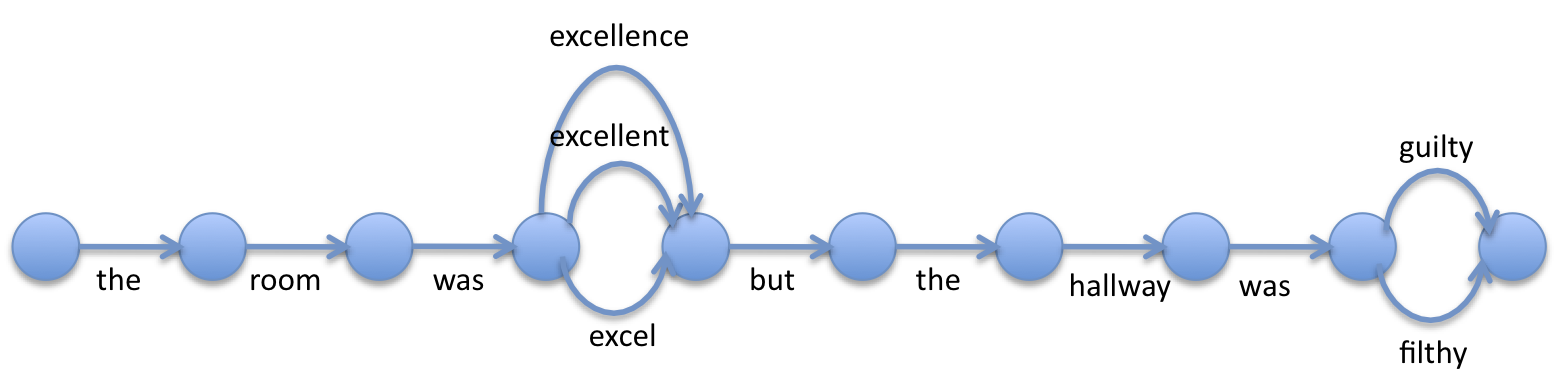
\includegraphics[scale=0.9]{confusion-network.png}\\[5mm]
Let the decoder decide
\end{center}

%%%%%%%%%%%%%%%%%%%%%%%%%%%%%%%%%%%%%%%%%%%%%%%%%%%%%%%%%%%%%%%%%%%%%%%%%%%%
\slide{Example: Diacritics}
\vspace{-3mm}
\begin{itemize}
\item Correct sentence \vspace{-5mm}
\begin{center}

\includegraphics[scale=0.8]{vietnamese.png}
\end{center}
\item Something a non-native person might type  \vspace{-2mm}
\begin{center}
	Trung Quoc canh bao My ve luat tien te
\end{center}

\item Confusion network \vspace{-8mm}
\begin{center}
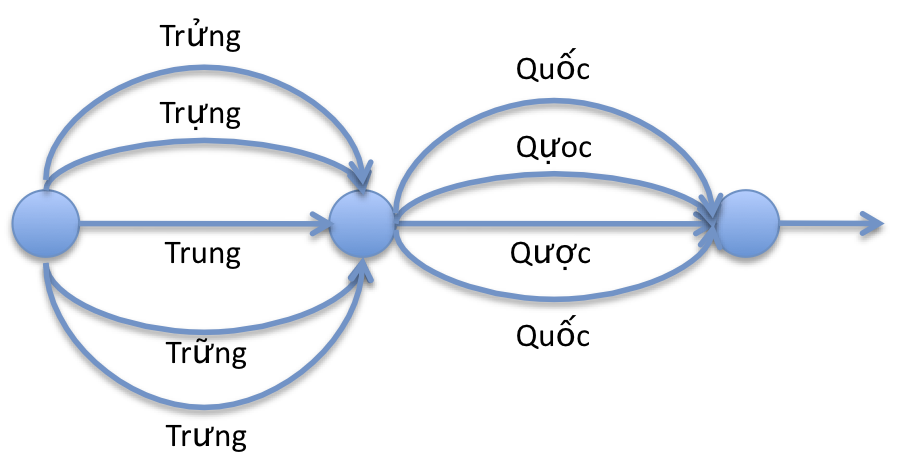
\includegraphics[scale=0.8]{confusion-network-2.png}
\end{center}
\end{itemize}

%Motivation - diacritics. 
% happens for many languages that have adapted roman characters. Can be used for arabic or hebrew - optional vowel characters

%%%%%%%%%%%%%%%%%%%%%%%%%%%%%%%%%%%%%%%%%%%%%%%%%%%%%%%%%%%%%%%%%%%%%%%%%%%%
\slide{Confusion Network Specification}
\begin{center}
\textcolor{red}{Argument on command line}\\[3mm]
\begin{SaveVerbatim}{myverb}
 ./moses -inputtype 1
\end{SaveVerbatim}
\colorbox{gray}{\BUseVerbatim{myverb}}

\vspace{10mm}
\textcolor{red}{Input to moses}\\[3mm]
{\small
\begin{SaveVerbatim}{myverb}
the 1.0
room 1.0
was 1.0
excel 0.33 excellent 0.33 excellence 0.33
but 1.0
the 1.0
hallway 1.0
was 1.0
guilty 0.5 filthy 0.5
\end{SaveVerbatim}
\colorbox{gray}{\BUseVerbatim{myverb}}}
\end{center}

%%%%%%%%%%%%%%%%%%%%%%%%%%%%%%%%%%%%%%%%%%%%%%%%%%%%%%%%%%%%%%%%%%%%%%%%%%%%
\slide{Lattice}
\begin{center}
\bf Example: Chinese Word Segmentation
\end{center}

\vspace{5mm}
\begin{itemize}
\item  Unsegmented sentence
\vspace{-5mm}
\begin{center}

\includegraphics[scale=1]{chinese-unsegmented.png}
\end{center}

\item  Incorrect segmention
\vspace{-5mm}
\begin{center}

\includegraphics[scale=1]{chinese-segmented-incorrect.png}
\end{center}

\item  Correct segmention
\vspace{-5mm}
\begin{center}

\includegraphics[scale=1]{chinese-segmented-correct.png}
\end{center}

\end{itemize}

%Follow on from confusion network.
%Motivation - chinese segmentation


%%%%%%%%%%%%%%%%%%%%%%%%%%%%%%%%%%%%%%%%%%%%%%%%%%%%%%%%%%%%%%%%%%%%%%%%%%%%
\slide{Lattice}
\vspace{20mm}
\begin{center}
Input to decoder:\\[10mm]
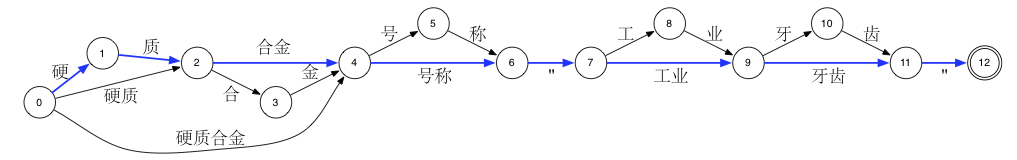
\includegraphics[scale=1.4]{lattice-chinese.png}\\[10mm]
Let the decoder decide
\end{center}

%%%%%%%%%%%%%%%%%%%%%%%%%%%%%%%%%%%%%%%%%%%%%%%%%%%%%%%%%%%%%%%%%%%%%%%%%%%%

\slide{Example: Compound Splitting}
\begin{itemize}
\item Input sentence 
\begin{center}
\example{einen wettbewerbsbedingten preissturz}
\end{center}
\item Different compound splits
\begin{center}
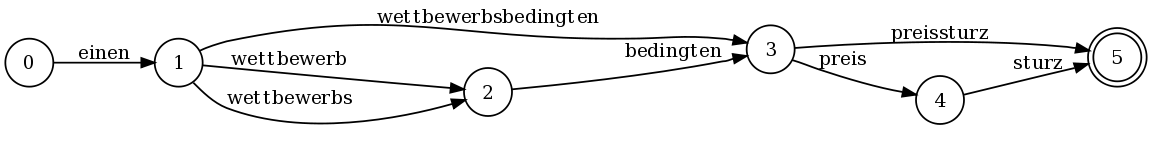
\includegraphics[scale=0.6]{lattice-german.png}
\end{center}
\item Let the decoder decide
\end{itemize}

% a competition-induced price fall
% german decompounding - unlikely to have seen many of the compund forms but have seen the separated words

%%%%%%%%%%%%%%%%%%%%%%%%%%%%%%%%%%%%%%%%%%%%%%%%%%%%%%%%%%%%%%%%%%%%%%%%%%%%
\slide{Lattice Specification}
\vspace{5mm}
%
%\begin{center}
%\textcolor{red}{Argument to command line}\\
%\begin{SaveVerbatim}{myverb}
% ./moses -inputtype 2
%\end{SaveVerbatim}
%\colorbox{gray}{\BUseVerbatim{myverb}}
%\end{center}

\begin{tabular}{ p{10cm}p{12cm} }
Command line argument & Input to Moses {\tiny (PLF format - Python Lattice Format)} \\
\vspace{-10.6cm}
\littlecode{./moses -inputtype 1} &
\tiny
\begin{SaveVerbatim}{myverb}
 (
  (
   ('einen', 1.0, 1),
  ),
  (
   ('wettbewerbsbedingten', 0.5, 2),
   ('wettbewerbs', 0.25, 1),
   ('wettbewerb', 0.25, 1),
  ),
  (
   ('bedingten', 1.0, 1),
  ),
  (
   ('preissturz', 0.5, 2),
   ('preis', 0.5, 1),
  ),
  (
   ('sturz', 1.0, 1),
  ),
 )
\end{SaveVerbatim}
\colorbox{gray}{\BUseVerbatim{myverb}}

\end{tabular}


%%%%%%%%%%%%%%%%%%%%%%%%%%%%%%%%%%%%%%%%%%%%%%%%%%%%%%%%%%%%%%%%%%%%%%%%%%%%

\slide{Advanced Features}
\vspace{-5mm}
\textcolor{darkgrey}{
\small
\begin{itemize} \itemsep -1mm
\item {How do I get started?}
\item {Experiment Management System}
\item {Faster Decoding}
\item {Data and domain adaptation}
\item {Instructions to decoder}
\item {Input formats}
\item \currenttopic{Output formats}
\end{itemize}
}

%%%%%%%%%%%%%%%%%%%%%%%%%%%%%%%%%%%%%%%%%%%%%%%%%%%%%%%%%%%%%%%%%%%%%%%%%%%%

\slide{N-Best List}

\begin{itemize}
\item Input \vspace{-5mm}
\begin{center}
\example{es gibt verschiedene andere meinungen .}
\end{center}

\item  Best Translation \vspace{-5mm}
\begin{center}
\example{there are various different opinions .}
\end{center}

\item  Next nine best translations \vspace{-5mm}
{\footnotesize \begin{center}
\example{
there are various other opinions . \\
there are different different opinions . \\
there are other different opinions . \\
we are various different opinions . \\
there are various other opinions of . \\
it is various different opinions . \\
there are different other opinions . \\
it is various other opinions . \\
it is a different opinions .}
\end{center}}
\end{itemize}

%%%%%%%%%%%%%%%%%%%%%%%%%%%%%%%%%%%%%%%%%%%%%%%%%%%%%%%%%%%%%%%%%%%%%%%%%%%%
\slide{Uses of N-Best Lists}
\vspace{20mm}
\begin{itemize}
\item  Let the translator choose from possible translations
\item  Reranker
	\begin{itemize}
	\item add more knowledge sources
	\item can take global view
	\item coherency of whole sentence
	\item coherency of document
	\end{itemize}
\item  Used to tune component weights
\end{itemize}

%n-best translations
%
%1. Best translation for the each input sentence
%2. 10-best translation for each input sentence
%- in sorted orde of best first
%      - think that the decoder can get good translation
%      - but not confident that the decoder will do a good job of finding the best translation.
%      - give 10 translations for the user to decide
%      
%      - in general, can ask the decoder to return the n-best sentences
%      
%      - more often used to give to a post-processing step. 
%      - let another algorithm decide which 1 really is the best sentence. Based on other critieria not in the decoder
%          - document level information.
%          
%          - pronoun translation from chinese/vietnamese to english.
%          - dependent on context.
%             -  no word for 'me'. Could be translated as nephew, uncle, grandfather, friend, depending on who you're talking to
%             -  'you' could be translated as nephew, uncle, grandfather, friend.
%   - external tools which looks at the whole document might do a better job finding the most appropriate. 
%   - give it 100-best translation, let it decide
% 

%%%%%%%%%%%%%%%%%%%%%%%%%%%%%%%%%%%%%%%%%%%%%%%%%%%%%%%%%%%%%%%%%%%%%%%%%%%%
\slide{N-Best Lists in Moses}
\vspace{5mm}
\begin{center}
Argument to command line\\[2mm]
\begin{SaveVerbatim}{myverb}
 ./moses -n-bestlist n-best.file.txt [distinct] 100
\end{SaveVerbatim}
\colorbox{gray}{\BUseVerbatim{myverb}}

\vspace{10mm}
Output\\[2mm]
{\footnotesize \begin{SaveVerbatim}{myverb}
0 ||| there are various different opinions .  ||| d: 0 lm: -21.6664 w: -6 ...  ||| -113.734
0 ||| there are various other opinions .  ||| d: 0 lm: -25.3276 w: -6 ... ||| -114.004
0 ||| there are different different opinions .  ||| d: 0 lm: -27.8429 w: -6 ...  ||| -117.738
0 ||| there are other different opinions .  ||| d: -4 lm: -25.1666 w: -6 ...  ||| -118.007
0 ||| we are various different opinions .  ||| d: 0 lm: -28.1533 w: -6 ...  ||| -118.142
0 ||| there are various other opinions of .  ||| d: 0 lm: -33.7616 w: -7 ...  ||| -118.153
0 ||| it is various different opinions .  ||| d: 0 lm: -29.8191 w: -6  ... ||| -118.222
0 ||| there are different other opinions .  ||| d: 0 lm: -30.426 w: -6 ...  ||| -118.236
0 ||| it is various other opinions .  ||| d: 0 lm: -32.6824 w: -6 ... ||| -118.395
0 ||| it is a different opinions .  ||| d: 0 lm: -20.1611 w: -6 ...  ||| -118.434

\end{SaveVerbatim}
\colorbox{gray}{\BUseVerbatim{myverb}}}
\end{center}

\slide{Acknowledgements}
\vspace{5mm}
\begin{table}[h]
\begin{center}
\begin{tabular}{ c  c  c } 


\includegraphics[scale=0.3]{univ-edinburgh.pdf}
&

\includegraphics[scale=0.07]{charles.png}
\\[1cm]

\includegraphics[scale=1]{fbk.png} 
&
\includegraphics[scale=0.6]{maryland.png}
\\[1cm]
\includegraphics[scale=1.5]{mit.png}
&
\includegraphics[scale=1]{aachen.png}
\end{tabular}
\end{center}
\end{table}

%%%%%%%%%%%%%%%%%%%%%%%%%%%%%%%%%%%%%%%%%%%%%%%%%%%%%%%%%%%%%%%%%%%%%%%%%%%%
\slide{Moses Developers}
\vspace{10mm}
\begin{center}
\footnotesize \rm
\begin{tabular}{cccc} 
Abhishek Arun & 
Adam Lopez & 
Ales Tamchyna & 
Alex \\
Amittai Axelrod &
Ankit Srivastava &
Anthony Rousseau &
Benjamin Gottesman \\ 
Barry Haddow &
Ondrej Bojar &
Chris Callison-Burch & 
Christine Corbett \\
Christian Hardmeier &
Christian Federmann &
Lane Schwartz &
David Talbot \\
Edmund Huber &
Evan Herbst &
Andreas Eisele &
Eva Hasler \\
Frederic Blain &
Brooke Cowan &
Grace M. Ngai&
Kenneth Heafield \\
Hieu Hoang &
H. Leal Fontes &
Holger Schwenk &
Josh Schroeder \\
Jean-Baptiste Fouet &
Joern Wuebker &
Jorge Civera &
Konrad Rawlik \\
Abby Levenberg &
Alexandra Birch &
Bo Fu &
M.J.Bellino-Machado \\
Mauro Cettolo &
Marcello Federico &
Michael Auli &
John Joseph Morgan \\
Mark Fishel &
Gabriele Antonio Musillo &
Miles Osborne &
Nadi Tomeh \\
Nicola Bertoldi &
Oliver Wilson &
Pascual Martinez &
Philipp Koehn \\
Phil Williams &
Bruno Pouliquen &
Raphael Payen &
Chris Dyer \\
Joao Luís Rosas &
Rico Sennrich &
Herve Saint-Amand &
Felipe Sanchez Martinez \\
Sara Stymne &
Steven B. Parks &
Steven Buraje Poggel &
Andre Lynum \\
Yizhao Ni &
David Kolovratnak &
Sergio Penkale &
Stephan \\
Suzy Howlett &
Wade Shen &
Yang Gao &
Tsuyoshi Okita \\
Alexander Fraser &
Richard Zens

\end{tabular}
\end{center}

%%%%%%%%%%%%%%%%%%%%%%%%%%%%%%%%%%%%%%%%%%%%%%%%%%%%%%%%%%%%%%%%%%%%%%%%%%%%
\end{document}
